% !TEX program = xelatex
\documentclass[bachelor,openright,notchinese]{sustcthesis}
% 默认twoside 双面打印
% 将master修改为bachelor, doctor or master
% 要使用adobe字体,添加adobefonts选项
% 使用euler数学字体,如不愿使用,去掉euler
% 使用外文写作,请添加notchinese

% 设置图形文件的搜索路径
\graphicspath{{figures/}}

% 用到的宏包
\makeatletter
\let\asme@citex\@citex % save amse2e definition of \@citex
\makeatother
\usepackage{algorithm2e}
\usepackage{url}
\makeatletter
\let\@citex\asme@citex % restore
\makeatother
% 阻止hyperref宏包影响tableofcontent内容
\makeatletter
\let\Hy@linktoc\Hy@linktoc@none
\makeatother

%%%%%%%%%%%%%%%%%%%%%%%%%%%%%%
%% 封面部分
%%%%%%%%%%%%%%%%%%%%%%%%%%%%%%
 % 中文封面内容
  \title{毕业论文}%一般情况下扉页和封皮、书脊共用一个标题文本,可以不用定义\spinetitle(仅硕博有用), \covertitle(本硕博均有用)和\encovertitle(仅本科有用)。特殊情况见下。
  %特殊情况1:本例中\title命令里含有换行控制字符,这会导致制作书脊的时候出现错误,例如如果你注释掉\spinetitle{...}这一行就会报错。这时需要定义一个不含换行等命令的\spinetitle,这并不表示\spinetitle里不能有任何命令——只能使用有限的命令。
  %特殊情况2:本例中标题过长,所以需要缩小书脊标题的字号。
  %特殊情况3:本例中中英文混排,由于tex竖排的原理限制,中英文基线不重合,所以需要人工调整英文的基线。具体调整量根据不同字体有所不同。
  %\covertitle{六次循环域}
  %\covertitle{中文题目第一行\\中文题目第二行}
  %不要在此调整封皮字体大小! Do not set Cover Page font size here!
  %特殊情况4:本例中\title中含有多个换行,导致标题超过了两行。根据制本厂规定,封皮标题不能超过两行。因此需要定义封皮使用的标题\covertitle. 如果你注释掉这一行,就会发现封皮不符合规定。
  %\encovertitle{On Cyclic Sextic Fields}
  %\encovertitle{English Title Line 1\\English Title Line 2\\English Title Line 3}
  %不要在此调整封皮字体大小! Do not set Cover Page font size here!
  %特殊情况5:仅本科生有用。本科封皮中有英文标题,不超过三行。与上类似。
  \author{李可明 }
  \depart{计算机科学与工程}%系别,硕博请用系代号,本科请用全称如
  \major{计算机专业}%专业,硕博请用全称,本科不需要
  \advisor{XXXX \ 教授}
  % \coadvisor{XXX\ 教授,\ XXX\ 教授}%第二导师,没有请注释掉
  \studentid{XXXXX}%For bachelor only
  \submitdate{二〇一九年三月}

  % 英文封面内容
  \entitle{Cover Ratio Maximization}
  \enauthor{Keming Li}
  \studentid{11612126}
  \endepart{Computer Science and Engineering}
  \enmajor{Computer Science and Technology}
  \enadvisor{Prof. Bo Tang}
  % \encoadvisor{}
  % \encoadvisorsec{}
  \ensubmitdate{May, 2020}
  
\begin{document}

% 封面
\maketitle

%特别注意,以下述顺序为准,在对应部分添加文档部件,切勿颠倒顺序:
%本科论文的文档部件顺序是:
%    frontmatter:致谢、目录、中文摘要、英文摘要、
%    mainmatter: 正文章节
%    backmatter: 参考文献或资料注释、附录
%%%%%%%%%%%%%%%%%%%%%%%%%%%%%%
%% 前言部分
%%%%%%%%%%%%%%%%%%%%%%%%%%%%%%
\frontmatter
\makeatletter

\ifustc@bachelor
	%%%%%%%%%%%%%%%%%
	%本科论文修改这里
	%%%%%%%%%%%%%%%%%
	% 致谢
	\chapter*{诚信承诺书}
\label{chap:honest}

\begin{enumerate}
\item 本人郑重承诺所呈交的毕业设计(论文),是在导师的指导下,独立进行研究工作所取得的成果,所有数据、图片资料均真实可靠。
\item 除文中已经注明引用的内容外,本论文不包含任何其他人或集体已经发表或撰写过的作品或成果。对本论文的研究作出重要贡献的个人和集体,均已在文中以明确的方式标明。
\item 本人承诺在毕业论文(设计)选题和研究内容过程中没有抄袭他人研究成果和伪造相关数据等行为。
\item 在毕业论文(设计)中对侵犯任何方面知识产权的行为,由本人承担相应的法律责任。
\end{enumerate}

\vskip 3\baselineskip


\begin{flushright}

作者签名: \underline{\hspace{4cm} 李可明}
\vskip \baselineskip
\underline{\hspace{1.4cm} 2020 }年\underline{\hspace{0.7cm} 5}月\underline{\hspace{0.7cm} 14}日

\end{flushright}



	%\chapter{Preface}
\label{chap:chap-preface}
\vskip 28pt

\begin{flushright}

Alan Mathison Turing

March, 2019 at SUSTech

\end{flushright}






     
	
	
	%目录部分
	%目录
	\tableofcontents
	%默认表格、插图、算法索引名称分别为“表格索引”、“插图索引”和“算法索引”
	%如果需要自行修改lot,lof,loa的名称,请定义
	%\ustclotname{...}
	%\ustclofname{...}
	%\ustcloaname{...}

	% 表格索引
	%\ustclot
	% 插图索引
	%\ustclof
	%算法索引 
	%如果需要使用算法环境并列出算法索引,请加入补充宏包。
	%\ustcloa
	
	% 摘要
	
\begin{enabstract}
    Decision making problem is popular among these days. In rank aware processing, 
    a user will only choose the option that ranks top-kF for himself. 
    Concretely, preferences of users are usually represented as weight vectors. 
    Each attribute of weight vector means how important is that attribute to that user. 
    The score of an option respecting to a user is the dot product between the user's 
    preference weight vector and the option. Only the options with top-k scores can 
    attract the user. An option covers a user if and only if it can rank top-k for 
    that user. Usually, a company has many products (options), each of which covers 
    some of the users. A user covered by a company means at least one of its products 
    covers this user. The company has to develop new product that satisfies a constraint 
    and make its all products including this new product cover as more users as possible. 
    In this paper, we study how to determinate which newly added option can maximize 
    the cover ratio of the company. This problem is essential in developing new product, 
    advertising, etc. We refer this problem as k-Cover Ratio Maximization. 
    In this paper, we begin from top-k problem's computational geometric nature using 
    Cell Tree to represented option spaces, and then from the relationship among constraint, 
    options and user preference weight vectors to more efficiently solve this problem 
    returning the exact optimal solution. We set a lot of experiments to show the efficiency
    of our optimizations and at the same time we found interesting relationship 
    between the constraint and running time. Combining with the experience of decision 
    making, we found that it is hard to tell what kinds of product could cover the most
    users when the constraint intersects with most the users top-k condition.

\enkeywords{User Cover ratio, Introduce new option, Top-k query, Weight vector}
\end{enabstract}

\begin{cnabstract}
近年来关于如何做决策的问题十分热门。在排名处理系统中, 会假设一个用户只会从排入他(她)
前k的产品中作出选择。 具体地, 用户对于产品各种属性的爱好会用权重向量来表示。权重向量每个维度的
大小表现了该维度对于该用户的重要性。一个产品的对于一个用户的分数就是产品的各个指标得分组成的向量
与该用户的权重向量的点乘。只有排进该用户前k的产品才有可能影响用户最后的选择。当且仅当一个用户的
产品排该用户前k时我们称该产品覆盖这个用户。对于一个公司, 它可能有很多产品, 每个产品都有各自的
覆盖用户群。 当公司的至少一款产品能覆盖某个用户时, 我们称该公司用户覆盖该用户。随着市场以及自身业
务的发展, 公司要研发一款新的满足一定约束条件的产品, 使得公司的所有产品包括新产品总的尽可能覆盖
最多的用户。在本篇论文中我们会讨论如何精确找到这个能使公司覆盖率最大的新产品。 
本篇论文讨论的问题在例如研发一款怎么样的新产品让公司总收益最大, 如何加强广告宣传使总覆盖用户最多
等非常多领域都有很大的应用价值, 同时我们把这个问题命名为k-Cover Ratio Maximization。
在本篇论文中, 我们从前k问题的计算几何性质入手用Cell Tree这种数据结构表达候选的产品空间, 
然后从约束条件、产品、用户、前k条件等内在联系做优化大大提高解决问题效率, 最后返回最优解的解集。
我们做了许多实验证明我们的优化的有效性,同时发现了运行效率与约束条件的关系, 与现实决策结合
得出在付出成本与成为大多数人前k的条件相交时是比较难决定什么样的产品会覆盖更多的用户的。

\keywords{用户覆盖率, 新产品决策, 前k查询, 权重向量}
\end{cnabstract}



%此文件中含有中英文摘要
   %\begin{denotation}
\item[$\mathbb{Q}$] rational number field
\end{denotation}

    
\else
	%%%%%%%%%%%%%%%%%
	%硕博论文修改这里
	%%%%%%%%%%%%%%%%%
	% 摘要
	
\begin{enabstract}
    Decision making problem is popular among these days. In rank aware processing, 
    a user will only choose the option that ranks top-kF for himself. 
    Concretely, preferences of users are usually represented as weight vectors. 
    Each attribute of weight vector means how important is that attribute to that user. 
    The score of an option respecting to a user is the dot product between the user's 
    preference weight vector and the option. Only the options with top-k scores can 
    attract the user. An option covers a user if and only if it can rank top-k for 
    that user. Usually, a company has many products (options), each of which covers 
    some of the users. A user covered by a company means at least one of its products 
    covers this user. The company has to develop new product that satisfies a constraint 
    and make its all products including this new product cover as more users as possible. 
    In this paper, we study how to determinate which newly added option can maximize 
    the cover ratio of the company. This problem is essential in developing new product, 
    advertising, etc. We refer this problem as k-Cover Ratio Maximization. 
    In this paper, we begin from top-k problem's computational geometric nature using 
    Cell Tree to represented option spaces, and then from the relationship among constraint, 
    options and user preference weight vectors to more efficiently solve this problem 
    returning the exact optimal solution. We set a lot of experiments to show the efficiency
    of our optimizations and at the same time we found interesting relationship 
    between the constraint and running time. Combining with the experience of decision 
    making, we found that it is hard to tell what kinds of product could cover the most
    users when the constraint intersects with most the users top-k condition.

\enkeywords{User Cover ratio, Introduce new option, Top-k query, Weight vector}
\end{enabstract}

\begin{cnabstract}
近年来关于如何做决策的问题十分热门。在排名处理系统中, 会假设一个用户只会从排入他(她)
前k的产品中作出选择。 具体地, 用户对于产品各种属性的爱好会用权重向量来表示。权重向量每个维度的
大小表现了该维度对于该用户的重要性。一个产品的对于一个用户的分数就是产品的各个指标得分组成的向量
与该用户的权重向量的点乘。只有排进该用户前k的产品才有可能影响用户最后的选择。当且仅当一个用户的
产品排该用户前k时我们称该产品覆盖这个用户。对于一个公司, 它可能有很多产品, 每个产品都有各自的
覆盖用户群。 当公司的至少一款产品能覆盖某个用户时, 我们称该公司用户覆盖该用户。随着市场以及自身业
务的发展, 公司要研发一款新的满足一定约束条件的产品, 使得公司的所有产品包括新产品总的尽可能覆盖
最多的用户。在本篇论文中我们会讨论如何精确找到这个能使公司覆盖率最大的新产品。 
本篇论文讨论的问题在例如研发一款怎么样的新产品让公司总收益最大, 如何加强广告宣传使总覆盖用户最多
等非常多领域都有很大的应用价值, 同时我们把这个问题命名为k-Cover Ratio Maximization。
在本篇论文中, 我们从前k问题的计算几何性质入手用Cell Tree这种数据结构表达候选的产品空间, 
然后从约束条件、产品、用户、前k条件等内在联系做优化大大提高解决问题效率, 最后返回最优解的解集。
我们做了许多实验证明我们的优化的有效性,同时发现了运行效率与约束条件的关系, 与现实决策结合
得出在付出成本与成为大多数人前k的条件相交时是比较难决定什么样的产品会覆盖更多的用户的。

\keywords{用户覆盖率, 新产品决策, 前k查询, 权重向量}
\end{cnabstract}



%此文件中含有中英文摘要
	% 目录
	\tableofcontents
	%默认表格、插图、算法索引名称分别为“表格索引”、“插图索引”和“算法索引”
	%如果需要自行修改lot,lof,loa的名称,请定义
	%\ustclotname{...}
	%\ustclofname{...}
	%\ustcloaname{...}

	% 表格索引
	\ustclot
	% 插图索引
	\ustclof
	%算法索引 
	%如果需要使用算法环境并列出算法索引,请加入补充宏包。
	%\ustcloa
	
	%符号说明,需要加入补充包
	\begin{denotation}
\item[$\mathbb{Q}$] rational number field
\end{denotation}
%不是必需的,如果不想列出请注释掉
\fi
\makeatother

%%%%%%%%%%%%%%%%%%%%%%%%%%%%%%
%% 正文部分
%%%%%%%%%%%%%%%%%%%%%%%%%%%%%%
\mainmatter
  \chapter{INTRODUCTION}
\label{chp:introduction}
Take smartphone market as an example, there are different models of smartphones 
($D=$\{$r_1, r_2, ..., {r_m}$\}). Each model ($r_i=(r_i[1], r_i[2], ..., r_i[d])$) 
has different prices, pixels, battery capacities, cooling capacities and etc. 
Now a company $P$ owns $x$ models ($P=$\{$p_1, p_2, ..., p_x$\}$\in D$) 
and a user data set $W=$\{$w_1, w_2, ..., w_n$\}. Different users prefer in 
different aspects, for example some of them may prefer smartphones that with 
large battery capacity but some prefer those with better quality of screen, so each 
$w_i=(w_i[1], w_i[2], ..., w_i[d])$ represents the preference weight vector corresponding 
to a single user. The score of a model $r_i$ respecting to a user $w_i$ is the 
dot product $r_i\cdot w_i$. Usually a user will only make a choice from his own 
view of top-$k$, so a product ranks top-$k$ for the users is quite important. 
A product covers a user only when its score ranks top-$k$ among all existing 
products $D$. With the development of company and market, company has to develop a new 
product to cover more users and make more profit. But with the limitation of technology, 
money and other factors, one can't develop a perfect product to cover all users. 
It can only develop a product that covers as more user as possible under a constraint. 
For a company, some of its products have covered some users, so what it wants to do 
is how to make this new product cover more users that uncovered before.

In real life, k-Cover Ratio Maximization ($kCRM$) can solve the problems that how to 
decide the next generation product for companies. In advertising industry, it can help 
merchants how to cover specific group such as students, pregnant women and children. 
Besides it can tell advertiser where to set up new advertising board and if do so it 
can cover which group of people. Data analysts can use it to discover which group of 
people is ignored by the market. It can tell vedio makers to make which kinds of vedios
to attract users in YouTube, TikTop or other vedio platform.

Generally speaking, it is not a product covers a user but a group of products covers 
a user. And for different users, there are different groups of products. Among these 
groups of products, there are uncertain number of identity products. In our problem, 
we are aim to find this new product in continuous product space, which means there are 
infinite candidate products, so it is difficult to tell which product covers the most 
users.

In this paper, we will use computational geometric nature of $kCRM$ to explain how to 
find the exact optimal options (products) with the data structure $CellTree$ mentioned 
in $kSPR$\cite{tang_mouratidis_yiu_2017}. Besides, from some observations of this problem, we propose advance 
method that ignore irrelevant users and candidate products to save time. At last 
we sample products that satisfy the constraint and use their maximal cover count to 
prune the $CellTree$.

	
  %自行添加
  \chapter{RELATED WORK}
\label{chap:related}
Based on the summary of $kSPR$\cite{tang_mouratidis_yiu_2017}, 
preference-based querying which based on the value of each attribute of products
are mainly two kinds, skyline \cite{borzsony_kossmann_stocker, papadias_tao_fu_seeger_2005, Efficient_Progeressive, kossmann_ramsak_rost_2002}
and top-$k$ query 
\cite{chang_bergman_castelli_li_lo_smith_2000, hristidis_papakonstantinou_2004, prefer, towards_robust, zou_chen_2008}. 
Skyline is also named as non-dominated set 
\cite{996017}, 
which including all 
the data that each of them isn't dominated by any other data in the dataset. "X dominates Y" 
means X is better them or equivalent to Y in all dimensions and there is at least one dimension 
that X is better than Y. In our paper, we are more closed to top-$k$ query.  Top-$k$ query 
will return $k$ products such that their scores are ranking top-$k$ respecting to the 
input user. Our problem is to find the region that where the new product lies 
will it rank top-$k$ for most of the rest given users. Another related problem is 
reverse top-$k$ \cite{vlachou_doulkeridis_xx, vlachou_doulkeridis_kotidis_norvag_2010, vlachou_doulkeridis_kotidis_norvag_2011}, 
which is to return the users that input product can rank top-$k$ 
respecting to them. Based on the output of top-$k$ query, why-not top-$k$ query 
\cite{6268270} is proposed
to change the user weight vector by advertisements, correcting wrong user information or other ways
with the minimum penalty to make an input product ranks top-$k$.  At the same time, 
based on the output of reverse top-$k$ query, why-not reverse top-$k$ query
\cite{gao_liu_chen_zheng_zhou_2015} is proposed to how to change the $k$ in top-$k$, 
the user weight vector $w$ or the product $p$'s attribute values so as to make $w$ shown in 
the reverse top-$k$ result of $p$.  


One of the related studies for our problem is $k-hit$ query\cite{peng_wong_2015}, which 
attempts to find 
$k$ products from given product dataset so as to rank top-1 of users as more as 
possible. The candidate solution of $k-hit query$ is discrete and finite while $kCRM$ 
is to 
find a new product ranks top-$k$ for as more users as possible.  At the same time, 
$CRM$ may return unknown number optimal products or even infinite products from continuous 
candidate space if only 
they are all optimal at the same time. 


A recent study $TopRR$\cite{tang_mouratidis_yiu_chen_2019} is very closed to our 
problem, which is attempting to return 
the product region that each of whose products can rank top-$k$ for all input users. 
The major different between $TopRR$ and $kCRM$ is that the candidate space is not complete 
in the domain of product for $kCRM$ since $kCRM$ can only choose the product that 
satisfies the constraint, 
which means in most cases, the optimal products can't cover all users and it is unknown
that the optimal products will cover how many or which users. 


In our paper, we use the $CTA$ approach as mentioned in $kSPR$ as our baseline. $kSPR$
is to return the user region that an input product can rank top-$k$ and it uses
a data structure $CellTree$ to exactly identify in which user space the product's score is
better than product dataset's another product's score, so $CellTree$ can take the regions that 
the input product not worse than other k products as results and return them. 
For $kCRM$, we transform our problem into return the product region that covers input users 
as more as possible. We find that to cover one or multiple users 
product also lies in regions and $CellTree$ can store and process them either. $CellTree$
will record each region cover how many users and return the region covers the most 
users as $kCRM$'s answer.   
 

 



  \chapter{PROBLEM DEFINITION}
\label{chap:chap-two}

In this section, we will firstly introduce related concept and then propose our 
problem.  

{\bfseries Definition 1.} A product $p$'s score respecting to a user $w$ is the 
dot product $p\cdot w$.

Without loss of generality, $w$ satisfies $w[i]\in [0, 1]$, $p$ satisfies 
$p[i]\in [0, 1]$ and $\Sigma_{i=1}^d w[i]=1$. We also take the values as larger
as better for products and so the larger the score the better.

{\bfseries Definition 2.} A product $p$ covers a user $w$ when the score 
respecting to $w$ ranks top-$k$ among $D$.

{\bfseries Problem 1.} The $k-Cover Ratio Maximization$ takes product dataset 
$D$, $P\subset D$, user data set $W$ and a positive integer $k$ as inputs. 
It introduces how to determine a new product $p$ such that satisfies the 
constraint $C(p)\leq B$ and maximizes the cover ratio of $P\cap \{p\}$:  
\begin{displaymath}
  cp(p, P, k)=\frac{|\left\{w|\forall w\in W, \left\{P\cup\left\{p \right\}\right\}\cap TopK(w)\neq \emptyset  \right\}|}{|W|}  
\end{displaymath}

For the sake of convenient, we define constraint $C(p)\leq B$ as $\Sigma_{i=1}^d p[i] \leq B$.
  \chapter{GEOMETRIC COMPUTATION NATURE}
\label{chap:chap-three}

\section{To Cover Users}
{\bfseries Definition 3.} The $k_{th}$ score $S_{ik}$ represents the scores 
to ranks top-k corresponding to user $w_i$. 

For simplicity, we mark 
\begin{enumerate}
    \item $w_i\cdot p=S_{ik}$ as $h_i$
    \item $w_i\cdot p>S_{ik}$ as $h_i^+$
    \item $w_i\cdot p<S_{ik}$ as $h_i^-$
\end{enumerate}

\begin{figure}[hbt!]
  \centering
  \begin{subfigure}[b]{0.45\linewidth}
    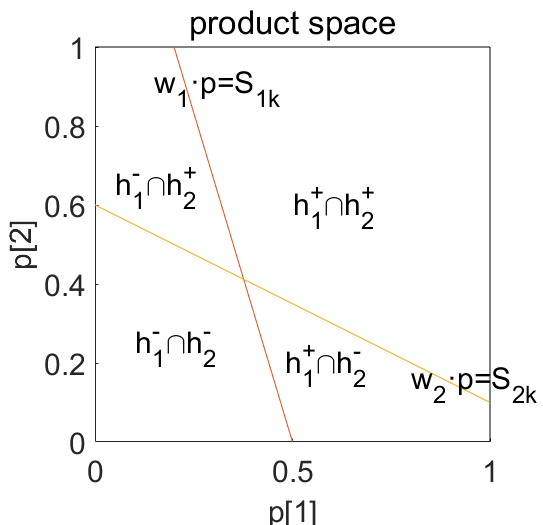
\includegraphics[width=\linewidth]{the_hp_insertion.png}
    \caption{Hyper-plane insertion}
    \label{the_hp_insertion}
  \end{subfigure}
  %
  \begin{subfigure}[b]{0.45\linewidth}
    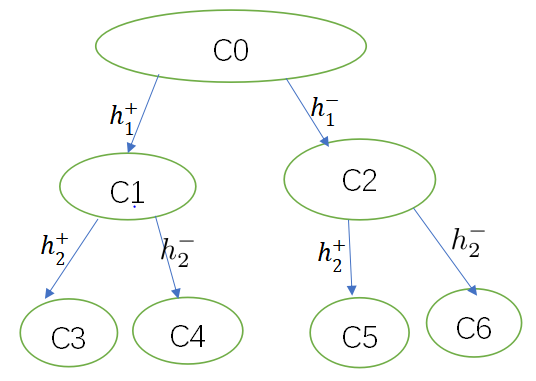
\includegraphics[width=\linewidth]{f2.png}
    \caption{$CellTree$ insertion}
    \label{cell_tree_nodes}
  \end{subfigure}
  \caption{hyper-plane insertion and $CellTree$ insertion}
\end{figure}

As shown in Figure \ref{the_hp_insertion}, when it comes to multiple users, 
such as 2 users
 $\{w_1, w_2\}$, firstly $h_1$ divides product space into 2 half-space 
 $h_1^+$ and $h_1^-$; then $h_2$ divides $h_1^+$ into $h_1^+\cap h_2^+$ 
 and $h_1^+\cap h_2^-$ and divides $h_1^-$ into $h_1^-\cap h_2^+$ and 
 $h_1^-\cap h_2^-$. 
Region $h_1^+\cap h_2^+$ covers both $w_1$ and $w_2$; region $h_1^+\cap h_2^-$  
could only cover $w_1$; region $h_1^-\cap h_2^+$ could only cover $w_2$; 
region $h_1^+\cap h_2^-$ can't cover any user.

\section{Cell Tree Representation}
The tree in Figure \ref{cell_tree_nodes} is called $CellTree$, which is firstly 
proposed by $kSPR$. We use the root node to represent the whole candidate space. 
After the insertion of $h_1$, the root node (cell) $c_0$ generates 2 child cells 
$c_1$ and $c_2$ while the space is divided into 2 parts; 
$c_1$ and $c_2$ represent $h_1^-$ and $h_1^-$ respectively. 
After the insertion of $h_2$, the cell $c_1$ generates 2 child cells $c_3$ and $c_4$; the cell $c_2$ generates 2 child cells $c_5$ and $c_6$. From root cell $c_0$ to cell $c_3$, we can clearly see that $c_3$ is $h_1^+\cap h_2^+$, which means $c_3$ covers $w_1$ and $w_2$. Similarly, $c_4$ is $h_1^+\cap h_2^-$, which means $c_3$ covers $w_1$. Among all the cells, $c_3$ covers the largest number of users. If we change the root cell as $C(p) \leq B$ and remove all those users that already covered by $P$ then we can use $CellTree$ to solve $kCRM$.


\section{Baseline Solution}
In the below paragraph, we will introduce our baseline approach to get the optimal solution for $kCRM$, which follows these steps:
\begin{enumerate}
\item Calculate the top-k score $S_{ik}$ for each $w_i\in W$.
\item Find all the $w_i\in W$ that $P$ covers and mark their set as $W^*$.
\item Update $W=W-W^*$.
\item Using $CellTree$ to find the cell that with maximal cover count and return the optimal cells. 
\end{enumerate}

\section{Time Comlexity}
\label{baseline_tc}
As proposed in $kSPR$, the $CellTree$ approach's time complexity is $O(n^d)$, which 
$n$ is the product dataset cardinality and $d$ is the dimensionalty of data.
For our problem, baseline solution time complexity is $O(n^d+nm\log m)$ or $O(n^d+nmk)$. 
$n$ means the cardinality of users that take part in $CellTree$ halfspace insertion. 
$d$ means the dimentionality of data.
$m$ means the cardinality of product dataset.
$O(nm\log m)$ is corresponding to the process of finding $S_{ik}$ for each user, which needs
calculating the dot product of users, sorting the scores and return the $k_{th}$ score.
We could also use seletion sorting instead of sorting methods with time complexity $O(m\log m)$
when product dataset is huge while $k$ is small to make getting $S_{ik}$ of all users
with time complexity $O(nmk)$.  
In most cases $n^d\gg nm\log m$, so we can take baseline's time complexity as $O(n^d)$.

\chapter{ADVANCE SOLUTION}
\label{chap:adva}

\section{Lemmas That Help to Prune}

Baseline solution basically is just a brute force method. Now we introduce some 
lemmas that prunes and accelerates the baseline solution.


{\bfseries Definition 4.} A product $p$ dominates another product $q$ 
if and only if $\forall i \in [1, d]$, the $i_{th}$ dimension $p[i] \geq q[i]$ and $\exists$ $i \in [1,d]$, the $i_{th}$ dimension $p[i]>q[i]$.

{\bfseries Lemma 1.} If  $\forall q$ that $C(q)<B, \exists p$ that $C(p)=B$ and $p$ dominates $q$, then there must be at least one optimal solution on $C(p)=B$.

Because for most of the constraint $C(p)<B$ is bounded by $C(p)=B$ and as for our defined 
constraint $\Sigma_{i=1}^d p[i] \leq B$ satisfies condition of Lemma 1, in 
experiments we only need to consider region $C(p)=B$ as our candidate space which is also the root node of $CellTree$.

On the base of Lemma 1 that only consider $C(p)=B$, which also means only $h_i$ will divide space 
$C(p)=B$ would affect where the optimal solutions are, we define Lemma 2.

{\bfseries Lemma 2.} Ignore the users $w$ such that $w\cdot p=S_k$ doesn't intersect with constraint $C(p)=B$ won't affect the $kCRM$ result.

\begin{figure}[hbt!]
  \centering
  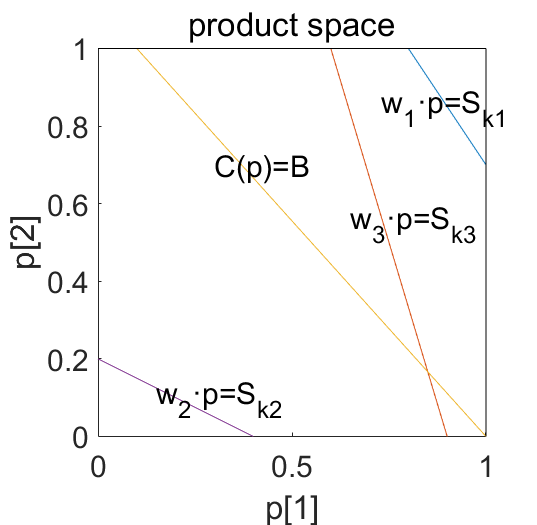
\includegraphics[width=.5\linewidth]{the_intersect.png}
  \caption{User Intersect With constraint}
  \label{explain_intersect}
\end{figure}

As shown in Figure \ref{explain_intersect}, if we decide to choose the new product
 from $C(p)=B$, we can see that $h_1$ also divides the product space into 2
  halfspaces, but all the products on $C(p)=B$ are in the “-” halfspace, 
  which means all of them can not cover $w_1$. 
  Different from $w_1$, the products that on $C(p)=B$ all can cover $w_2$. 
  From this observation, we can move out all the users $w$ such that 
  $w_i \cdot p=S_{ik}$ doesn't intersect with $C(p)=B$.


 
{\bfseries Definition 5.} The negative space count for a $CellTree$ node is the 
negative spaces from this node to root node traversing by ancestor node one by one.

Take Figure \ref{cell_tree_nodes} as an example, the negative space count
\begin{enumerate}
\item For cell $c_4$ is 1 because of $h_2^-$,
\item For cell $c_5$ is 1 because of $h_1^-$, 
\item For cell $c_6$ is 2 because of $h_1^-$ and $h_2^-$.
\end{enumerate}

{\bfseries Lemma 3.} If the cover count of optimal solution in $kCRM$ is at least 
$\beta $ and $card(W)=n$, then all the 
nodes with more than $n-\beta $  can't become the optimal solution and they can 
be pruned.

Lemma 3 means that if we can judge there is no solution in a space can become 
optimal solution because them can't cover at least $\beta$ users, then we can 
prune this space. Take Figure \ref{cell_tree_nodes} as example, if $\beta=2$ 
which means the optimal solution should at least cover 2 users 
and $W=\{w_1, w_2, w_3\}$, then the nodes $c_3$, $c_4$, $c_5$ can be pruned 
because they can never cover at least 2 users even after the insertion of 
$h_3$. Actually, $\beta$ is the lower bound of optimal solution.

{\bfseries Definition 6.} Pruning number $\alpha $ is defined as $\alpha = n-\beta $ 
which based on Lemma 3.

Pruning number $\alpha$ means that if a node's negative space count exceeds 
$\alpha$, than it is safe to prune this node.

\section{Get Pruning Number}
Based on Lemma 3, to find a proper $\beta$, we simply uniformly generate new 
products 
in candidate space and then find the maximal cover count of them.
The procedure is:
\begin{enumerate}
\item Uniformly generate new products $P'=$\{$p_{1}', ..., p_{y}'$\} on $C(p')=B$.
\item Calculate cover count of each of $P'$.
\item Find the maximal cover count of $P'$ as $\beta$
\item Pruning number $\alpha=card(W)-\beta$ 
\end{enumerate}



\section{Insertion Order of Users}

{\bfseries Definition 7.} Maximal likely cover count of a user means  
the maximal cover count of the sampled products that cover this user.

As mentioned in Lemma 3, we prune the cell nodes that with more that $\alpha$ 
negative halfspaces. 
To be earlier prune the nodes that itself and its sub-tree leaf nodes can't be 
optimal solution,
we can firstly insert the halfspace that its positive halfspace not likely be 
the component of optimal solutions.
Our method to determinate the insertion order of halfspace is by the maximal 
likely cover count of users (we write CoverCount in short as CC):

\begin{enumerate}
  \item Initialize the cover count of each user as 0.
  \item Uniformly generate new products $P'=$\{$p_{1}', ..., p_{y}'$\} on $C(p')=B$.
  \item for $p'$ in $P'$ 
  \begin{enumerate}
    \item $W'$ is the user set covered by $p$
    \item $p'.CC=card(W')$
    \item for $w'$ in $W'$
    \begin{enumerate}
      \item $w'.CC=max(w'.CC, p.CC)$
    \end{enumerate}
  \end{enumerate}
  \item update $W=AscendingSortByCC(W)$
  \item return $W$
\end{enumerate}


{\bfseries Lemma 4.} Insert users by the order of their maximal likely cover counts in ascending.

The assumption that proposes Lemma 4 is that we don't want those users positive 
halfspaces $h_i^i$
hide with the user positive halfspaces can be part of optimal because that would make 
us use $\alpha$ to prune nodes quit late for it has generate many nodes can't be
part of optimal solutions. 




\section{Summary of Lemmas}
\begin{enumerate}
    \item Lemma 1 prunes the candidate space from $C(p) \leq B$ to $C(p)=B$.
    \item Lemma 2 moves out the users $w$ that $w\cdot p=S_k$ doesn't intersect with $C(p)=B$
    \item Lemma 3 state that in the process of $CellTree$ we can prune the nodes whose negative space count is more than pruning number $\alpha$. 
    \item Lemma 4 introduces a heuristic trick that forces pruning some nodes using
    Lemma 3.   
  \end{enumerate}

\section{Advance Solution}
The main procedure for advance solution in short is:
\begin{enumerate}
  \item Remove users covered by $P$.
  \item Remove users by Lemma 2.
  \item Apply Lemma 4 change the insertion order of users' halfspace.
  \item Apply Lemma 1 on root node of $CellTree$.
  \item Apply Lemma 3 prune nodes when doing $CellTree$ insertion.
\end{enumerate}
For more details:
\begin{enumerate}
\item Calculate the top-$k$ score $S_{ik}$ for each $w_i\in W$.
\item Find all the $w_i\in W$ that $P$ covers, mark their set as $W^*$.
\item Update $W=W-W^*$.
\item Find all the $w_i\in W$ that $w_i\cdot p=S_{ik}$ doesn't intersect with $C(p)=B$, mark their set as $W^{**}$.
\item Update $W=W-W^{**}$.
\item Generate new products on candidate space and find their maximal cover count as $\beta$
\item Let pruning number $\alpha =card(W)-\beta $
\item Update candidate space from $C(p) \leq B$ to the part of $C(p)=B$.
\item Chnage order of users $W$ as defined in Lemma 4
\item For $w_i \in W$,
try to insert $h_i$ for existing $CellTree$ using depth first search.
\begin{enumerate}
\item If the current node is marked as pruned, return.
\item Else if the node is in $h_i^-$, increase its negative space count by 1.
\begin{enumerate}
  \item If the node's negative space count exceeds $\alpha$ mark it as pruned.
  \item Increase its sub-tree nodes' negative space count by 1.
\end{enumerate} 
\item Else if the node is in $h_i^+$, increase its child nodes' and its cover count by 1.
\item Else if there is no child nodes of current node, generate two child nodes as 
      $h_i^-$ and $h_i^+$, return. 
\item Else if two child nodes marked as pruned, the current node is also marked as pruned
\item Else traverse to its child nodes.
\end{enumerate}
\item Return the node with maximal cover count.
\end{enumerate}

\section{Time Complexity}
As memtioned in Section \ref{baseline_tc}, the baseline's time complexity is $O(n^d)$.
For advance solution, we reduce the candidate space from $C(p)\leq B$ to $C(p)=B$, 
which actually reduces our time complexity to $O(n^{d-1})$ because the candidate space
reduces by 1 dimension and the insertion halfspace reduces by 1 dimension together.
Besides, we remove the users that doesn't intersect with $C(p)=B$. Actually, some of these users
may related to the optimal solution, for example their halfspace may enclose
the optimal solution region but since we give up all the candidate space of 
$C(p)<B$ they then just look unrelated to the optimal solution. In fact, if we want
an optimal solution with the lower cost we need those users that $h_i^-$ are totally
cover by $C(p)\leq B$. Back to the thesis of this section, the $n$ in $O(n^{d-1})$
reduces users quit a lot. We use $n_{new}$ to represented the cardinality of 
user data after removing the user by Lemma 3, then our time complexity is $O(n_{new}^{d-1})$.


\chapter{EXPERIMENT RESULTS}
\label{chap:exp}


\section{Experiment Setting}


\begin{table}[hbt]
  \caption{Product data set}
  \label{tab: parameter1}
  \centering
  \begin{tabular}{c|c|c|c|p{5cm}}
    \toprule
    Dataset & d & n & Attributes & Source \\
    \midrule 
    \midrule
    HOTEL  & 4 & 186,637 & hotels-base.com& \parbox{5cm}{No. of stars,\\ No. of rooms, \\No. of facilities, \\Price} \\
    \midrule
    HOUSE  & 6 & 315,063& ipums.org & \parbox{5cm}{Gas, Electricity,\\ Water, Heating,\\ Insurance, Property tax} \\
  \bottomrule
\end{tabular}
\end{table}

\begin{table}[hbt]
  \caption{Experiment parameters and default setting}
  \label{tab: parameter2}
  \centering
  \begin{tabular}{c|c}
    \toprule
    Lemma 3 product samples & 10k, 100K, 1M, {\bfseries 10M}\\
    $card(P)$ &  0, 5000, {\bfseries 10000}, 15000, 20000 \\
    Product dataset & {\bfseries HOTEL}, HOUSE\\
    User data size   & 1000, {\bfseries 5000}, 10000      \\
    User data distribution  & {\bfseries Uniform}, Correlated, Anti-correlated  \\
    $k$ & 5, {\bfseries 10}, 20, 30 \\
    $B$ for HOTEL & 1, {\bfseries 1.25}, 1.5, 2 , 2.5, 3\\
    $B$ for HOUSE & 3, 3.5, 4 ,4.5, 5, 5.5 , 5.7 , 5.9\\
  \bottomrule
\end{tabular}
\end{table}

\begin{figure}[hbt!]
  \centering
  \begin{subfigure}[b]{0.45\linewidth}
    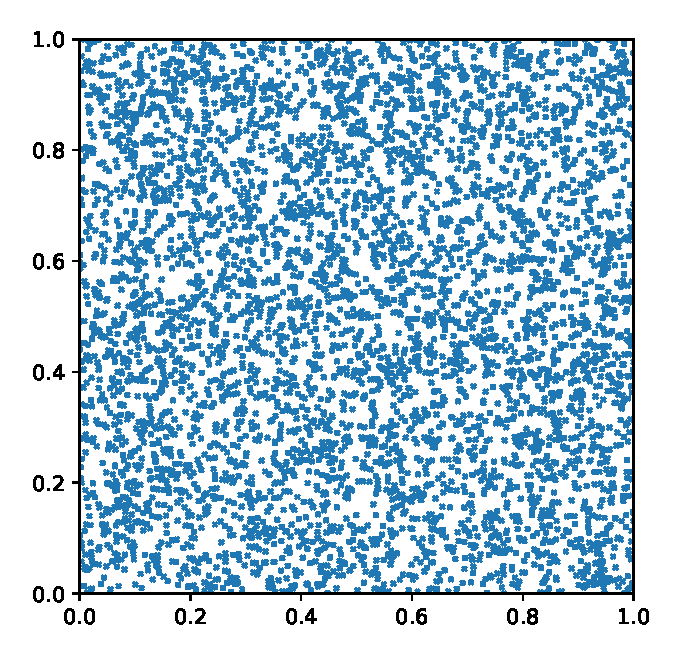
\includegraphics[width=.99\textwidth]{fig_uni}
    \caption{Uniform Distribution Data}
    \label{fig_uni}
  \end{subfigure}
  % %
  % \begin{subfigure}[b]{0.45\linewidth}
  %   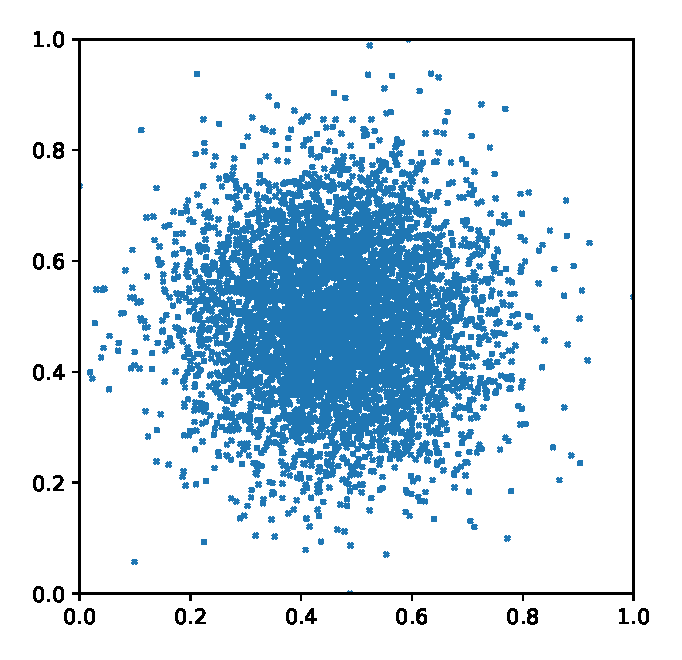
\includegraphics[width=.99\textwidth]{fig_gauss}
  %   \caption{Gaussian Distribution Data}
  %   \label{fig_gauss}
  % \end{subfigure}
  %
  \begin{subfigure}[b]{0.45\linewidth}
    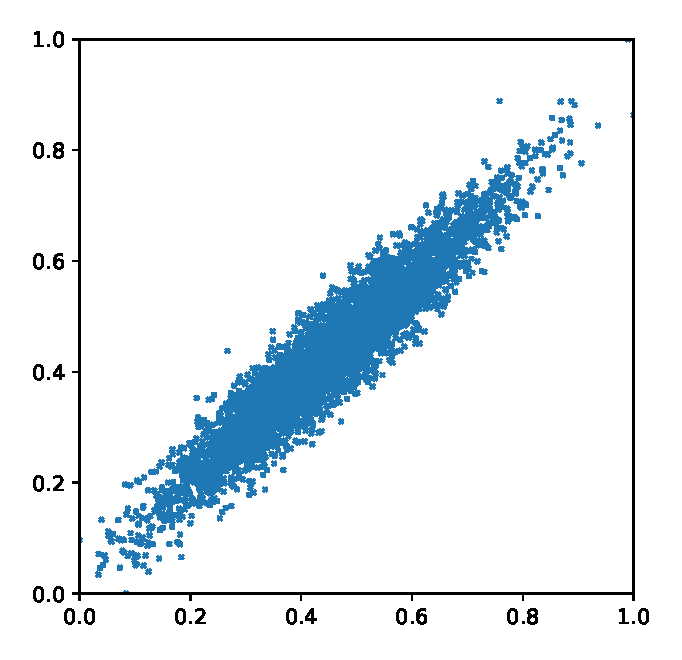
\includegraphics[width=.99\textwidth]{fig_corr}
    \caption{Correlated Distribution Data}
    \label{fig_corr}
  \end{subfigure}
  %
  \begin{subfigure}[b]{0.45\linewidth}
    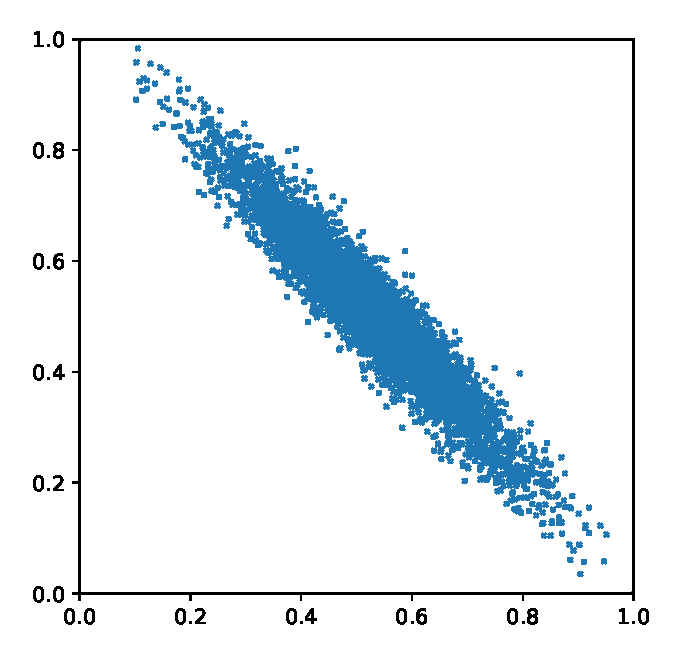
\includegraphics[width=.99\textwidth]{fig_anti}
    \caption{Anti-correlated Distribution Data}
    \label{fig_anti}
  \end{subfigure}
  \caption{Different Distribution Data in 2d}
  \label{data distribution}
\end{figure}

There are 3 kinds of datasets, the product data set $D$, $m=card(D)$; 
the product data set $P$, which uniformly generated by $D$ and so $P\subset D$;
the user data set $W$, all the attributes of data $w\in W$ satisfy $\Sigma w[i]=1$. 
The dimensionality of data is marked as $d$. 
Table \ref{tab: parameter1} shows all the product datasets. 
Table \ref{tab: parameter2} shows the parameters' setting and 
our default setting of them. Figure \ref{data distribution} shows how different
distribution data looks like. For example, if we want to sample products according
to correlated distribution with 2 attributes, then the final generated data will
looks like Figure \ref{fig_corr}.


All codes are implemented by C++; 
the procedure of insertion of $h_i$ needs LP solver and we use $lp\_solve$($http://lpsolve.sourceforge.net/5.5/$)
 to do it and the effciency of $lp\_solve$ has been proved by $kSPR$.  
The running machine is with Intel Xeon Gold 5122 - 3.60 GHz CPU, 128GB DDR4 RAM. 

\section{Effectiveness of Lemmas and Tricks}
In this section, we mainly discuss that how much does each lemma effetively help us
solve $kCRM$. And because there are some parameters within our advance algorithm, 
we would also explore how and why they could influence the efficiency of our algorithm
the way shown in our experiments.


\begin{figure}[ht!]
  \centering
  \begin{subfigure}[b]{0.45\linewidth}
    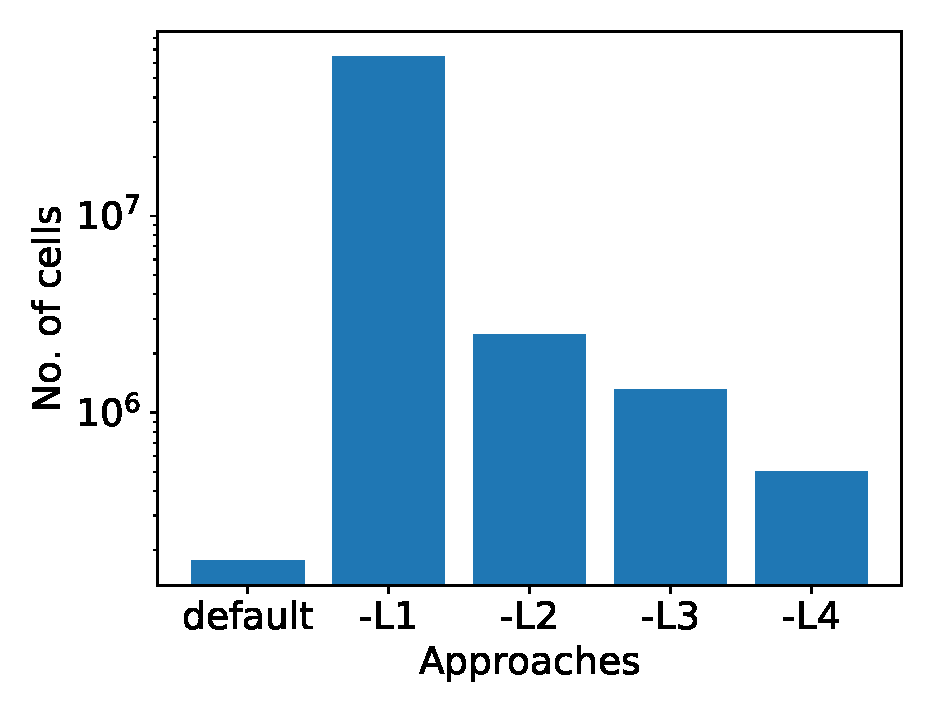
\includegraphics[width=.99\textwidth]{exp_lemmas1}
    \caption{No. of cells}
    \label{lemmas_on_cell}
  \end{subfigure}
  %
  \begin{subfigure}[b]{0.45\linewidth}
    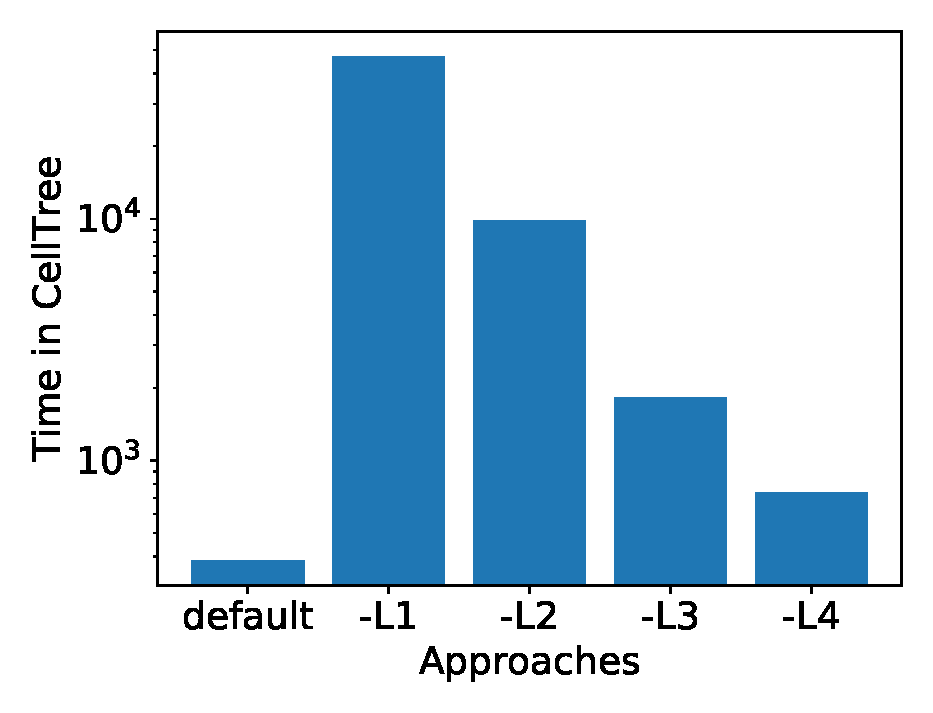
\includegraphics[width=.99\textwidth]{exp_lemmas2}
    \caption{Time spent in $CellTree$}
    \label{lemmas_on_time}
  \end{subfigure}
  \caption{Effectiveness of Lemmas}
  \label{lemmas}
\end{figure}

Firstly, we would show a global view of each lemmas as in Figure \ref{lemmas}.
-L1 means for advance solution, we apply $C(p)\leq B$ instead of $C(p)=B$ and 
the other optimization will be remained. For -L2, it will take account with those 
users $w_i$ such that $w_i\cdot p=S_{ik}$ doesn't intersect with $C(p)=B$. 
For -L3, it won't generate any lower bound of optimal solution or anything related
to pruning number $\alpha$ and it will just do insertion in $CellTree$ no matter how 
many negative spaces the nodes in. For -L4, it will randomly insert users into $CellTree$.
The default running means, we will
\begin{itemize}
  \item only consider $C(p)=B$
  \item remove unrelated users respecting to $C(p)=B$
  \item sample new product on $C(p)=B$, get lower bound of optimal solution and 
  then use $\alpha$ to prune nodes in $CellTree$.
  \item based on the less likely to be one of the covered users of optimal solution to insert 
  users so as to earlier prune them. 
\end{itemize}


As shown in Figure \ref{lemmas_on_cell}, because Lemma 1 tells that we only take account 
$C(p)=B$, which means we reduce most of the candidate space and reduce problem from 
$d$ dimension to $d-1$ dimension, it will improve our approach by hundreds of times of cells and running time. 
For the other lemmas, it also improves our algorithm by dozens of times.


\begin{figure}[ht!]
  \centering
  \begin{subfigure}[b]{0.45\linewidth}
    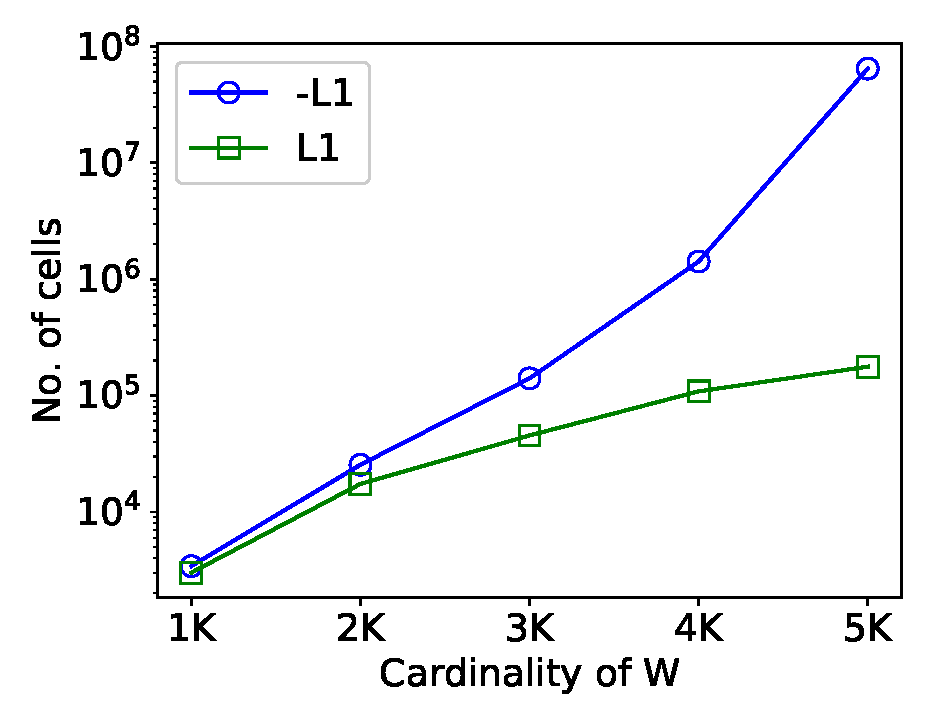
\includegraphics[width=.99\textwidth]{exp_L1_0}
    \caption{No. of cells}
    \label{exp_L1_0}
  \end{subfigure}
  %
  \begin{subfigure}[b]{0.45\linewidth}
    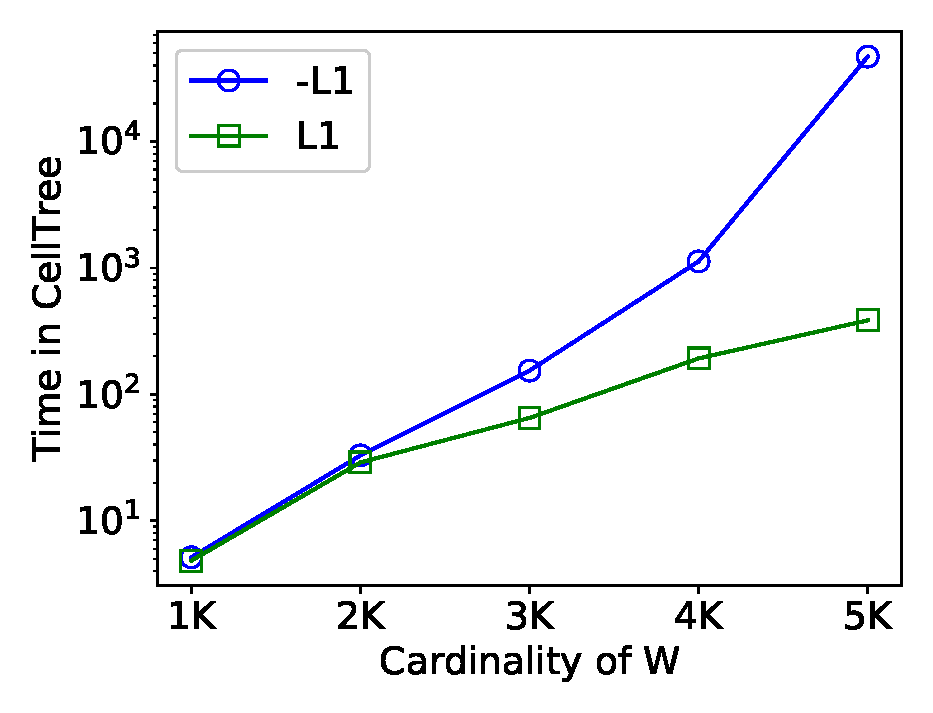
\includegraphics[width=.99\textwidth]{exp_L1_1}
    \caption{Time spent in $CellTree$}
    \label{exp_L1_1}
  \end{subfigure}
  \caption{Effectiveness of Lemma 1}
  \label{exp_L1}
\end{figure}

\begin{figure}[ht!]
  \centering
  \begin{subfigure}[b]{0.45\linewidth}
    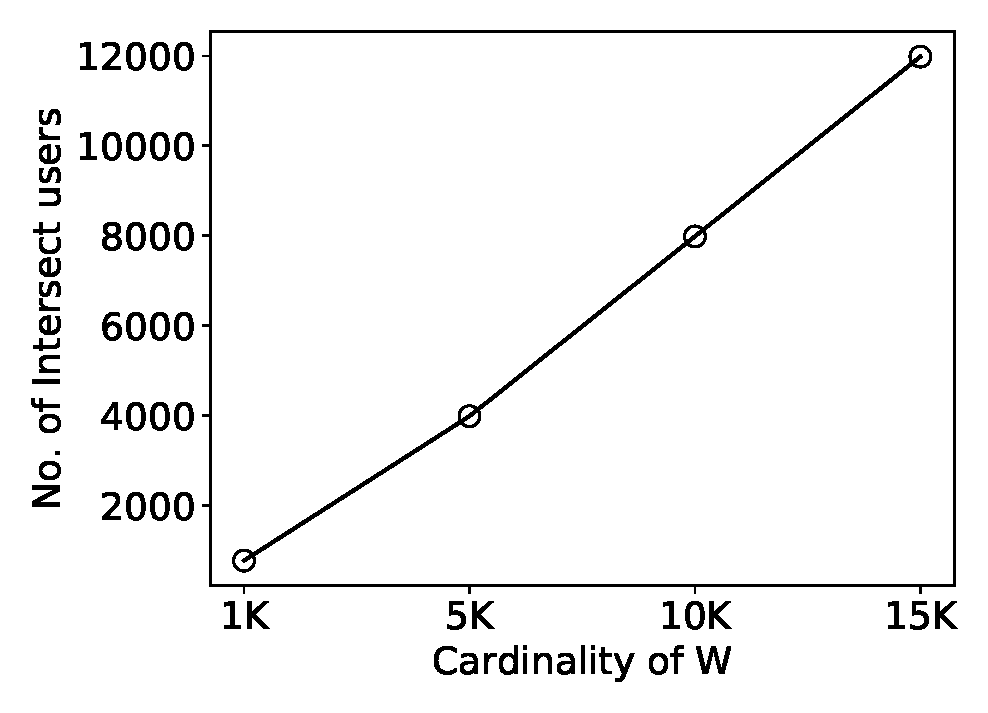
\includegraphics[width=.99\textwidth]{exp_L2}
    \caption{No. of cells}
    \label{exp_L2_in}
  \end{subfigure}
  \caption{Effectiveness of Lemma 2}
  \label{exp_L2}
\end{figure}

\begin{figure}[ht!]
  \centering
  \begin{subfigure}[b]{0.45\linewidth}
    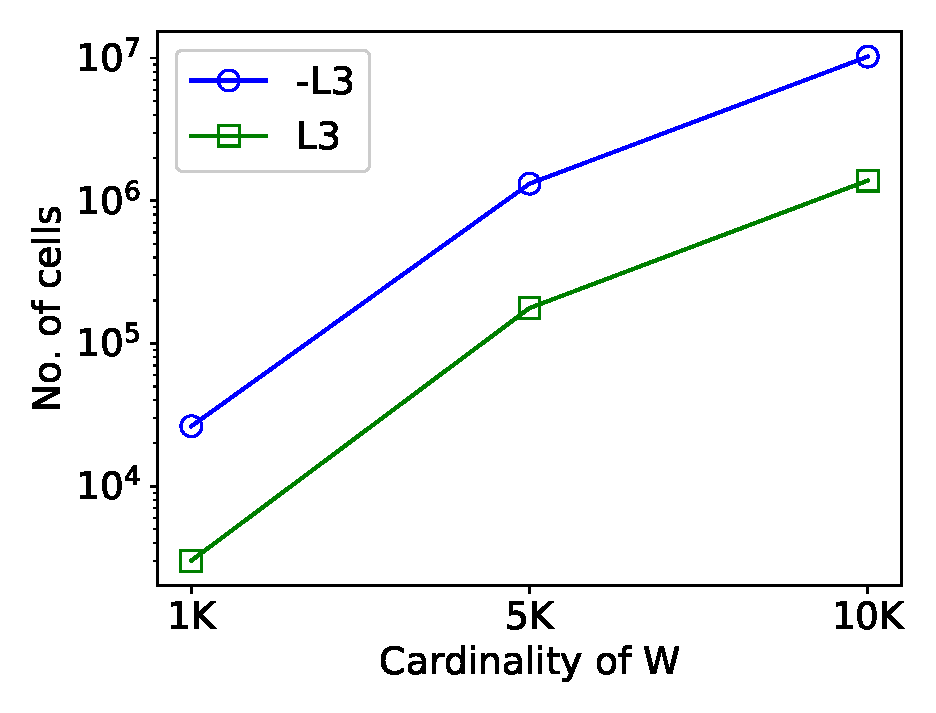
\includegraphics[width=.99\textwidth]{exp_L3_0}
    \caption{No. of cells}
    \label{exp_L3_0}
  \end{subfigure}
  %
  \begin{subfigure}[b]{0.45\linewidth}
    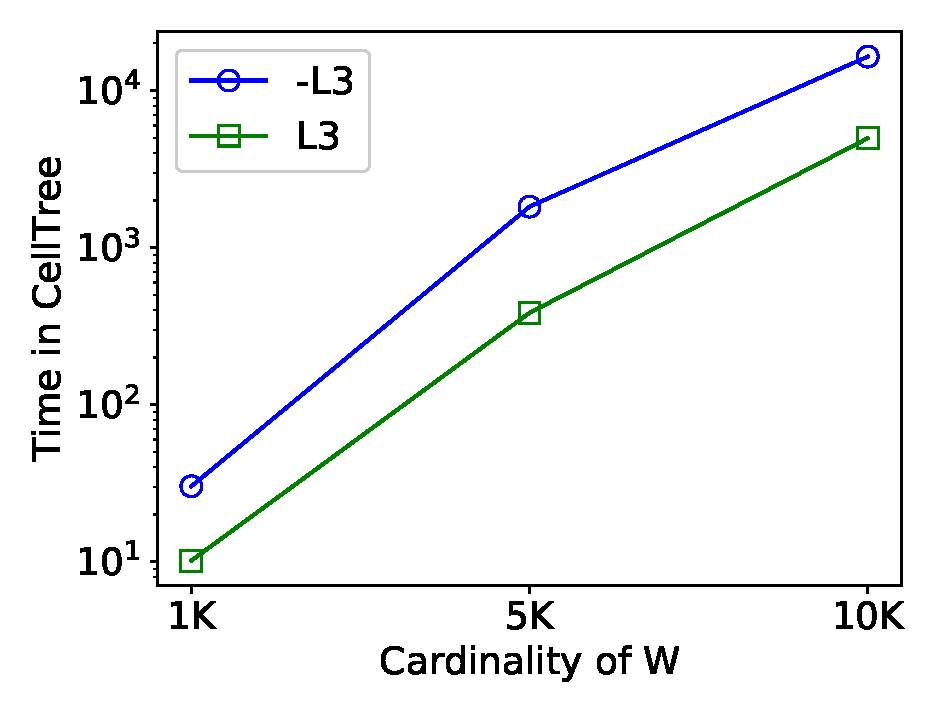
\includegraphics[width=.99\textwidth]{exp_L3_1}
    \caption{Time spent in $CellTree$}
    \label{exp_L3_1}
  \end{subfigure}
  \caption{Effectiveness of Lemma 3}
  \label{exp_L3}
\end{figure}

\begin{figure}[ht!]
  \centering
  \begin{subfigure}[b]{0.45\linewidth}
    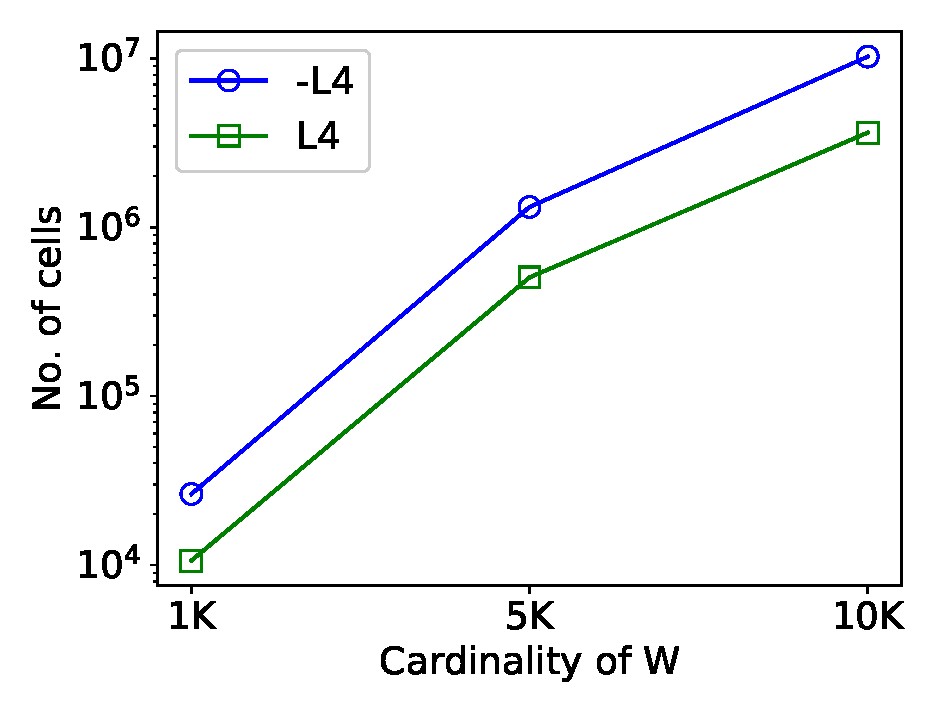
\includegraphics[width=.99\textwidth]{exp_L4_0}
    \caption{No. of cells}
    \label{exp_L4_0}
  \end{subfigure}
  %
  \begin{subfigure}[b]{0.45\linewidth}
    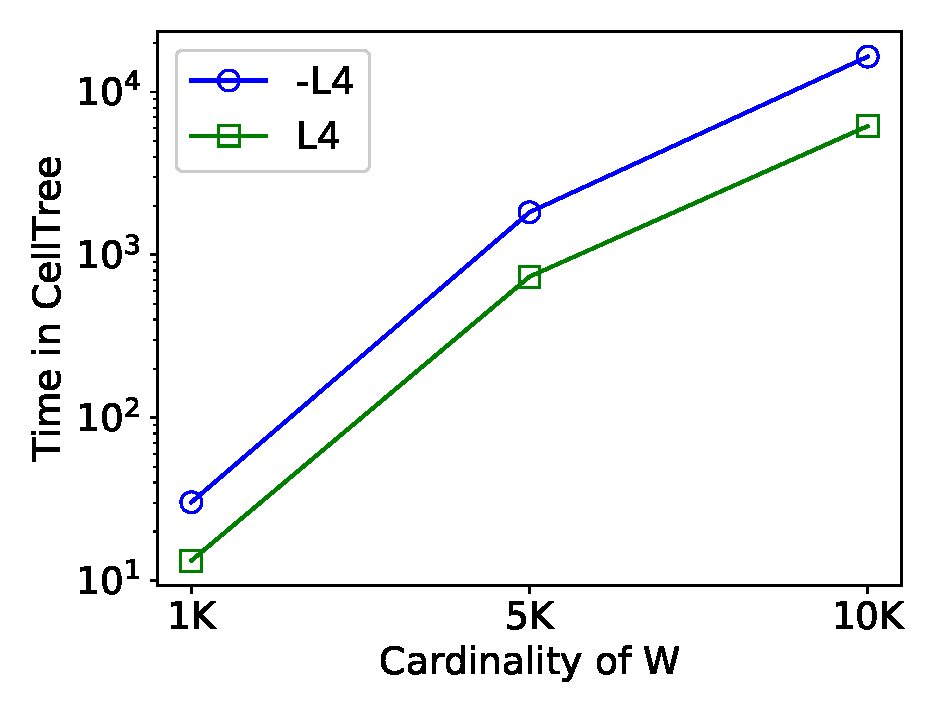
\includegraphics[width=.99\textwidth]{exp_L4_1}
    \caption{Time spent in $CellTree$}
    \label{exp_L4_1}
  \end{subfigure}
  \caption{Effectiveness of Lemma 4}
  \label{exp_L4}
\end{figure}

\begin{figure}[ht!]
  \centering
  \begin{subfigure}[b]{0.45\linewidth}
    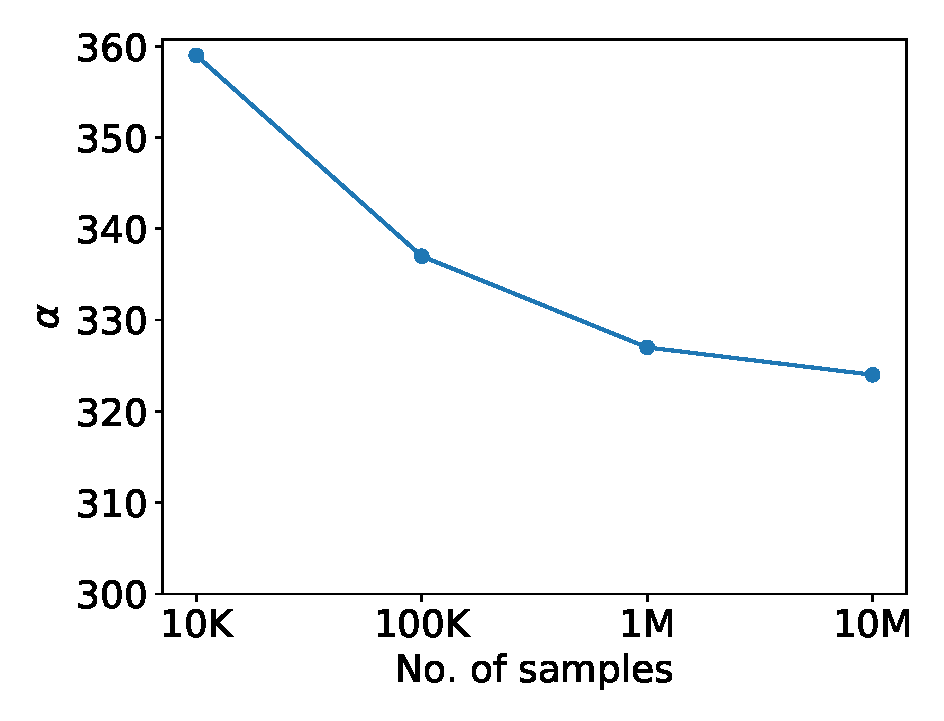
\includegraphics[width=.99\textwidth]{exp_sampleCnt0}
    \caption{pruning number $\alpha$}
    \label{newpdtcnt_on_alpha}
  \end{subfigure}
  %
  \begin{subfigure}[b]{0.45\linewidth}
    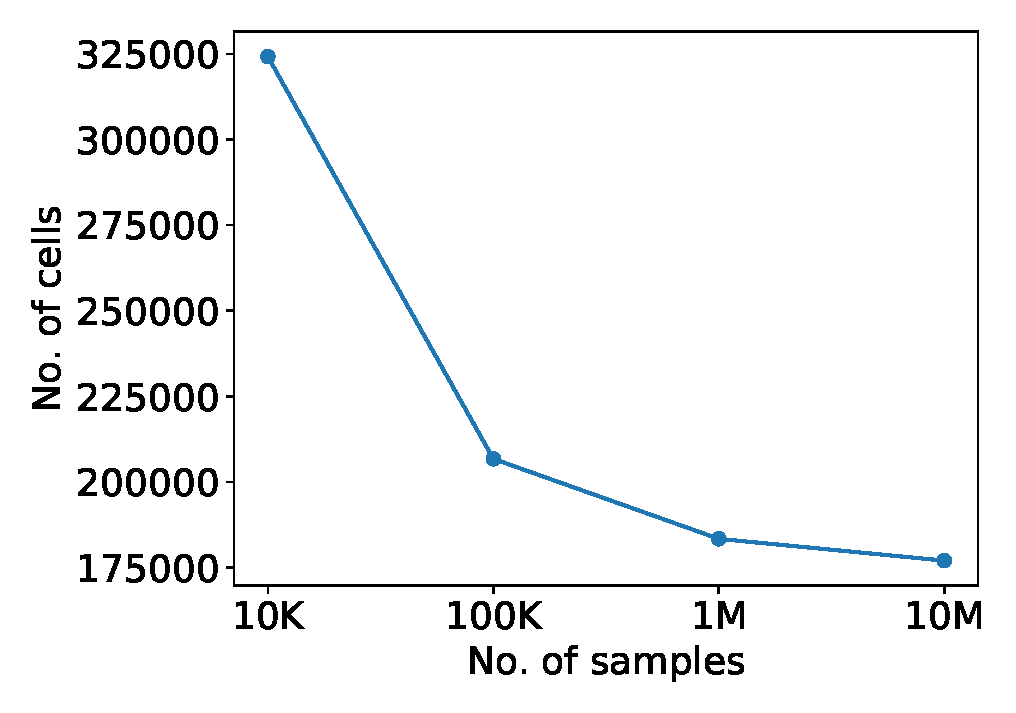
\includegraphics[width=.99\textwidth]{exp_sampleCnt1}
    \caption{No. of cells}
    \label{newpdtcnt_on_cell}
  \end{subfigure}
  %
  \begin{subfigure}[b]{0.45\linewidth}
    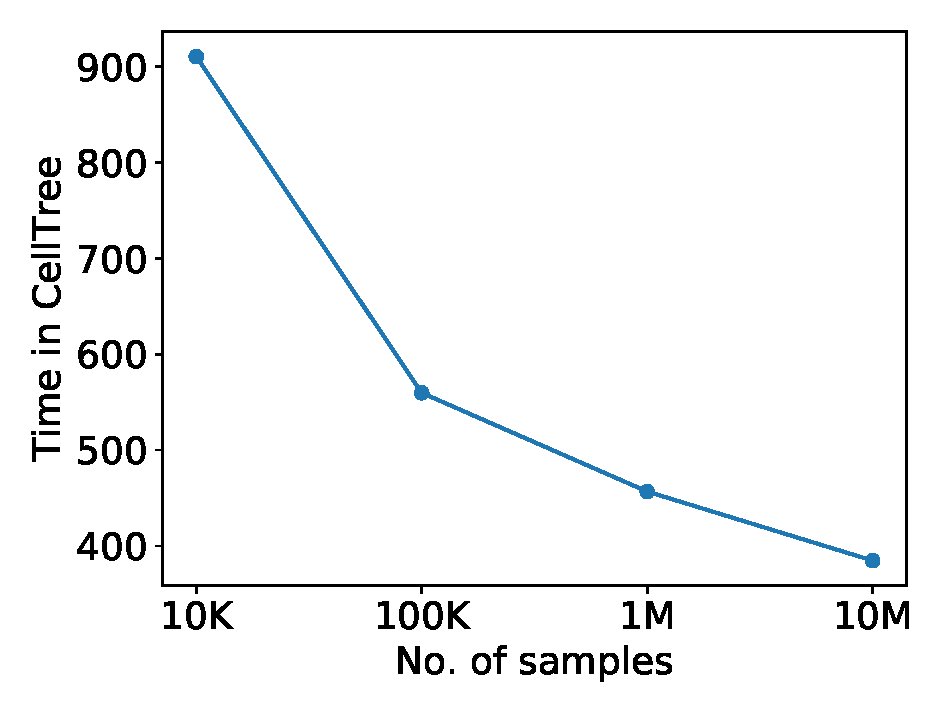
\includegraphics[width=.99\textwidth]{exp_sampleCnt2}
    \caption{Time spent in $CellTree$}
    \label{newpdtcnt_on_time}
  \end{subfigure}
  \caption{Effect of No. of newly sampled products}
  \label{lemma3_cnt}
\end{figure}

For each of lemmas, we make some experiments for details of how efficient they are.
In Figure \ref{exp_L1}, $-L1$ means when the situation without applying Lemma 1 but 
keeping the other lemmas work. With the change of cardinality of user dataset $W$,
$CellTree$'s cell number and running time grow fast for $-L1$ while grow more slower
for $L1$. In Figure \ref{exp_L2}, we skip the previous step that remove the users 
that covered by $P$ and clearly see that the number users, whose $w_i\cdot p=B$ 
would intersect constraint $C(p)=B$, grows linearly with cardinality of $W$. 
In Figure \ref{exp_L3}, we applying other lemmas but without Lemma 3, which 
using lower bound of optimal solution to prune tree cells of $CellTree$, comparing
applying Lemma 3 shows that Lemma 3 help us save space and time efficiently. Figure
\ref{exp_L4} also shows the effectiveness of Lemma 4 which changes the insertion order of
users to $CellTree$ in order to earlier prune the nodes that unlikely to be the
ancestor cell of optimal solution nodes.


In Lemma 3 we say that we would sample new products on $C(p)=B$ to get pruning number and 
next we will show the cardinality of newly generated new products influences our algorithm.
 The sampling time is negligible
for time in $CellTree$ insertion and we won't discuss the time spent by sampling in this section.
As shown in Figure \ref{newpdtcnt_on_alpha}, $\alpha$ slowly decreases with the increment of samples. 
We can also see from Figure \ref{newpdtcnt_on_cell} and Figure \ref{newpdtcnt_on_time} though
the change of $\alpha$ is small, but it makes a huge impact on resulting cells number in 
$CellTree$. This can explained by our algorithm's time complexity, $O(n^d)$, which means a 
litter change of users improves response time huge. 



\section{Influence of Inputs}
In this section, we would show the compact of input parameters to our algorithm. 

\begin{figure}[ht!]
  \centering
  \begin{subfigure}[b]{0.45\linewidth}
    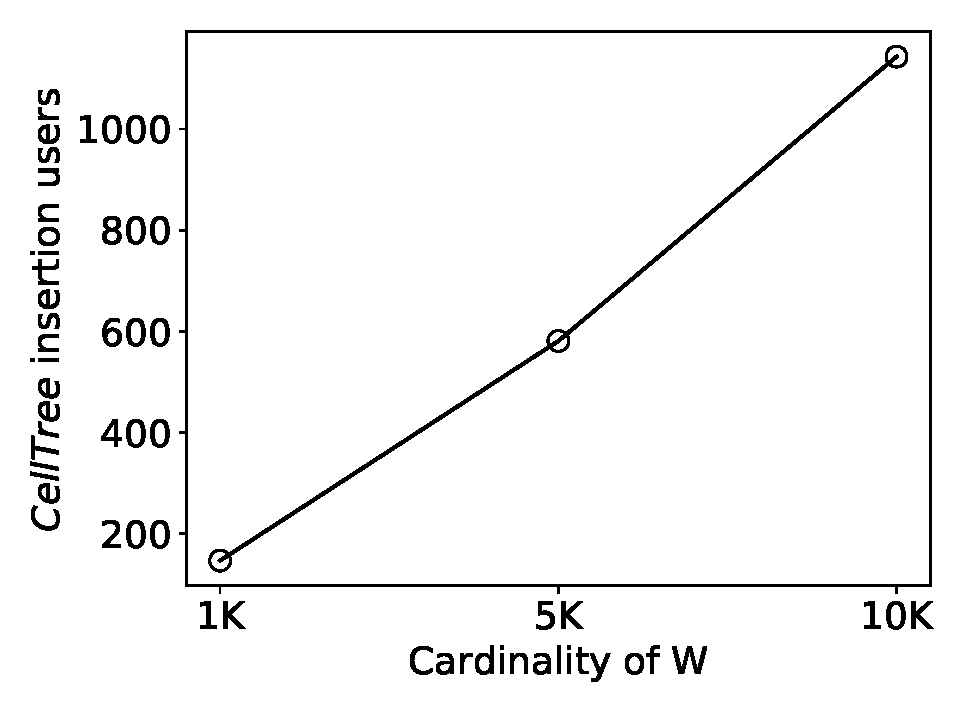
\includegraphics[width=.99\textwidth]{exp_cardW0}
    \caption{Processed users in $CellTree$}
    \label{exp_cardW0}
  \end{subfigure}
  %
  \begin{subfigure}[b]{0.45\linewidth}
    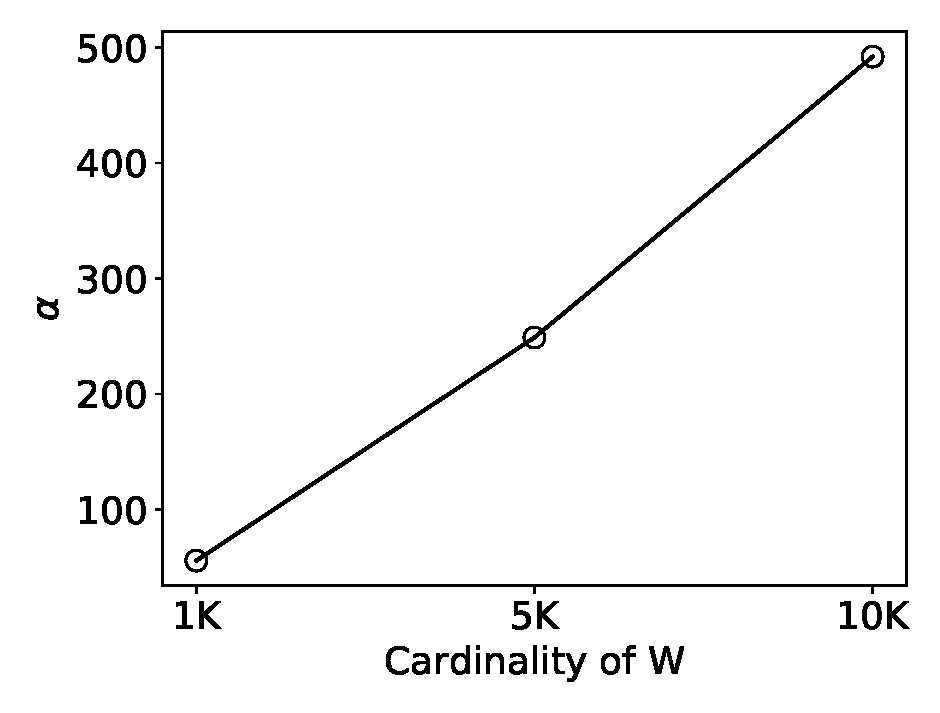
\includegraphics[width=.99\textwidth]{exp_cardW1}
    \caption{Pruning number $\alpha$}
    \label{exp_cardW1}
  \end{subfigure}
  %
  \begin{subfigure}[b]{0.45\linewidth}
    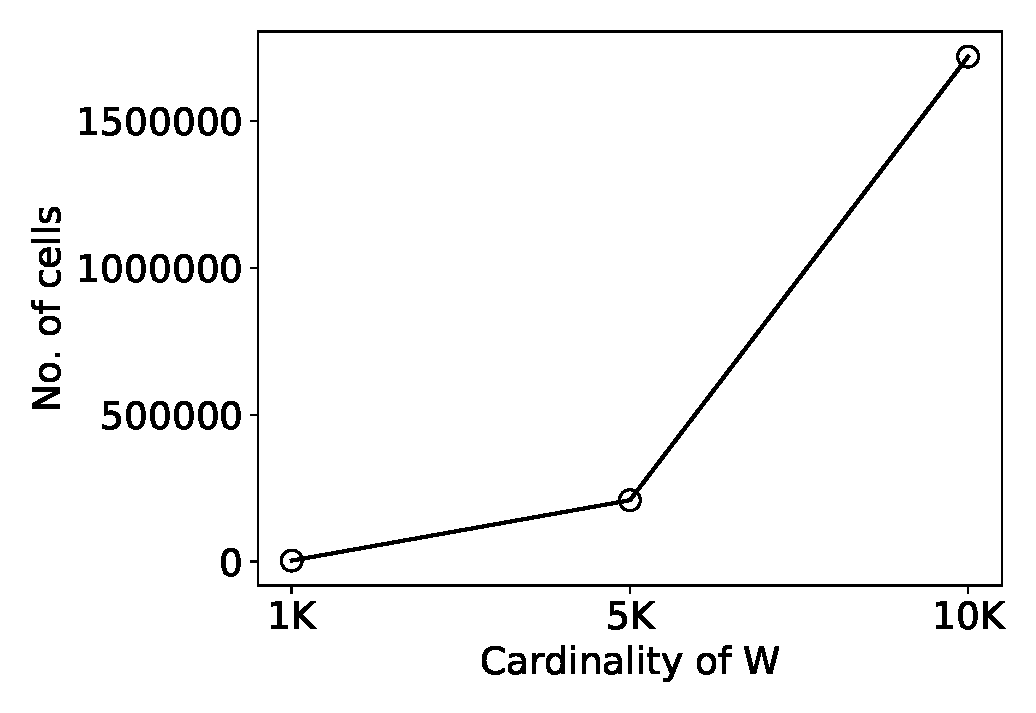
\includegraphics[width=.99\textwidth]{exp_cardW2}
    \caption{No. of cells}
    \label{exp_cardW2}
  \end{subfigure}
  %
  \begin{subfigure}[b]{0.45\linewidth}
    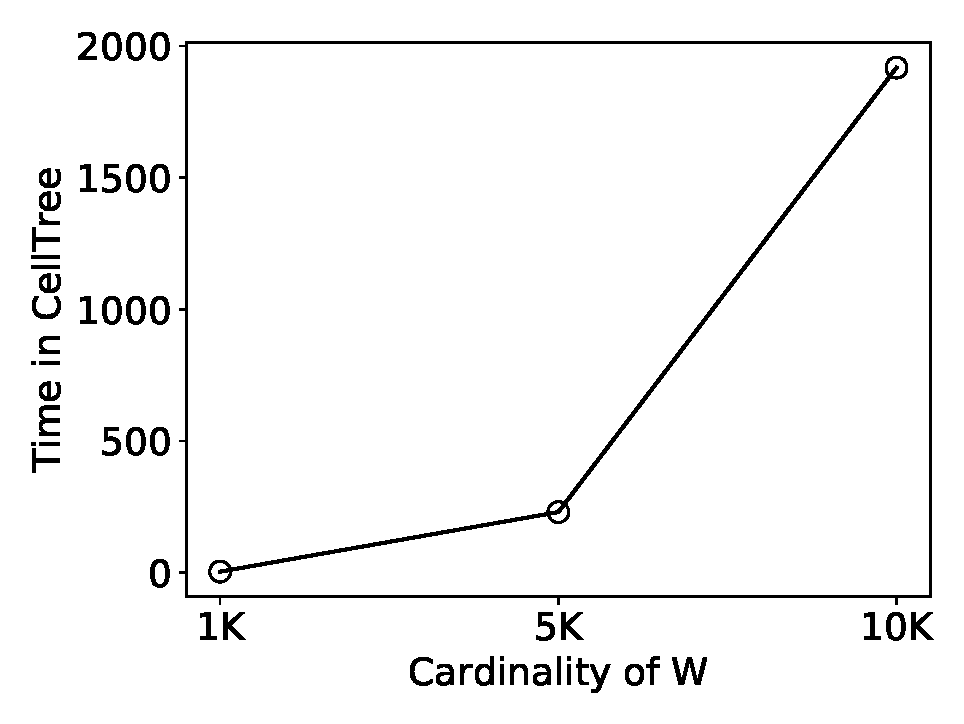
\includegraphics[width=.99\textwidth]{exp_cardW3}
    \caption{Time spent in $CellTree$}
    \label{exp_cardW3}
  \end{subfigure}
  \caption{Effect of cardinality of user dataset $W$}
  \label{cardW}
\end{figure}

Since the time complexity is $O(n^d)$, we can see from Figure \ref{cardW} that the users 
remain to be inserted in $CellTree$ grow linearly while the resulting cells and response 
time growing exponentially. 


\begin{figure}[hbt!]
  \centering
  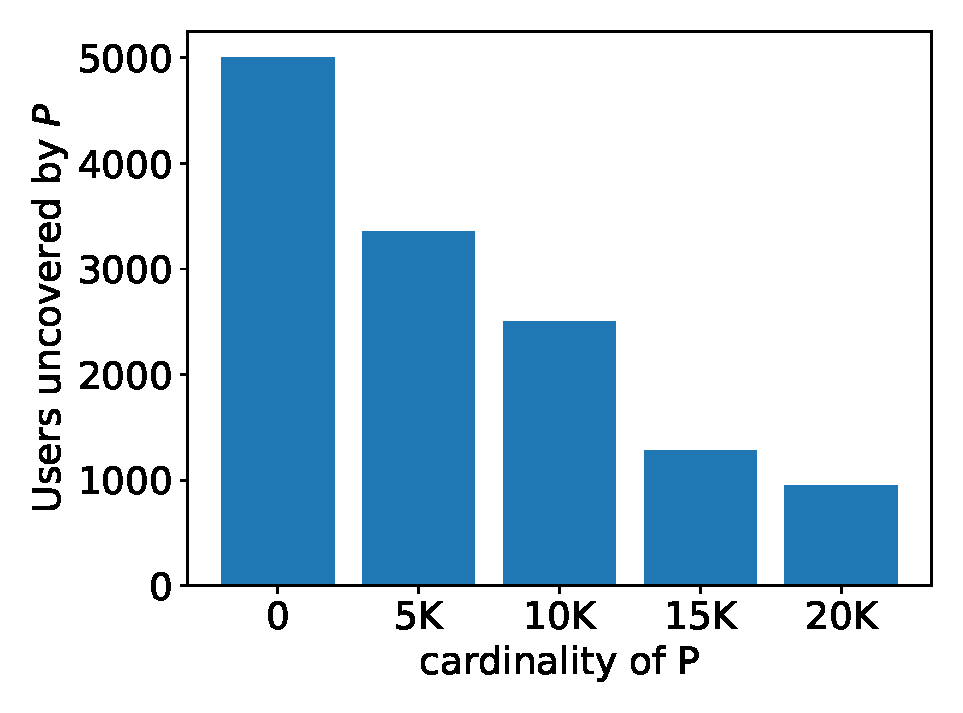
\includegraphics[width=.5\linewidth]{exp_lemmas0}
  \caption{Effect of $card(P)$ on user uncovered by $P$}
  \label{p_on_user}
\end{figure}
Product dataset $P$ will influence the efficiency of solving problems because in some
extreme condition, or unluckily $P$ only covers a few users; but sometime, $P$ will covers 
most of users. To complete the experiment of explore the global view impact of 
cardinality of $P$, we run 20 times sampling different $P$ for each attribute as shown in 
Figure \ref{p_on_user}. The original user data sizes are all 5000 and are the same. The y
axis means how many users is left that uncovered by $P$. We can see from Figure 
\ref{p_on_user} such that with the increment of cardinality of $P$, uncovered 
users number decreases slower and slower. 



\begin{figure}[ht!]
  \centering
  \begin{subfigure}[b]{0.45\linewidth}
    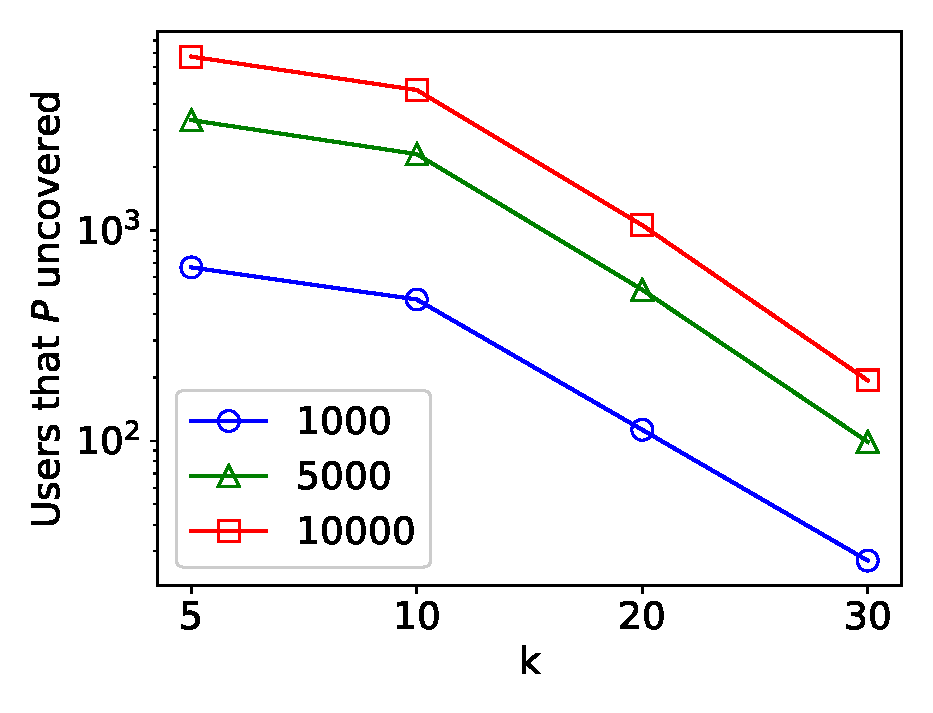
\includegraphics[width=.99\textwidth]{exp_topk0}
    \caption{User uncovered by $P$}
    \label{k_change_user_cnt}
  \end{subfigure}
  %
  \begin{subfigure}[b]{0.45\linewidth}
    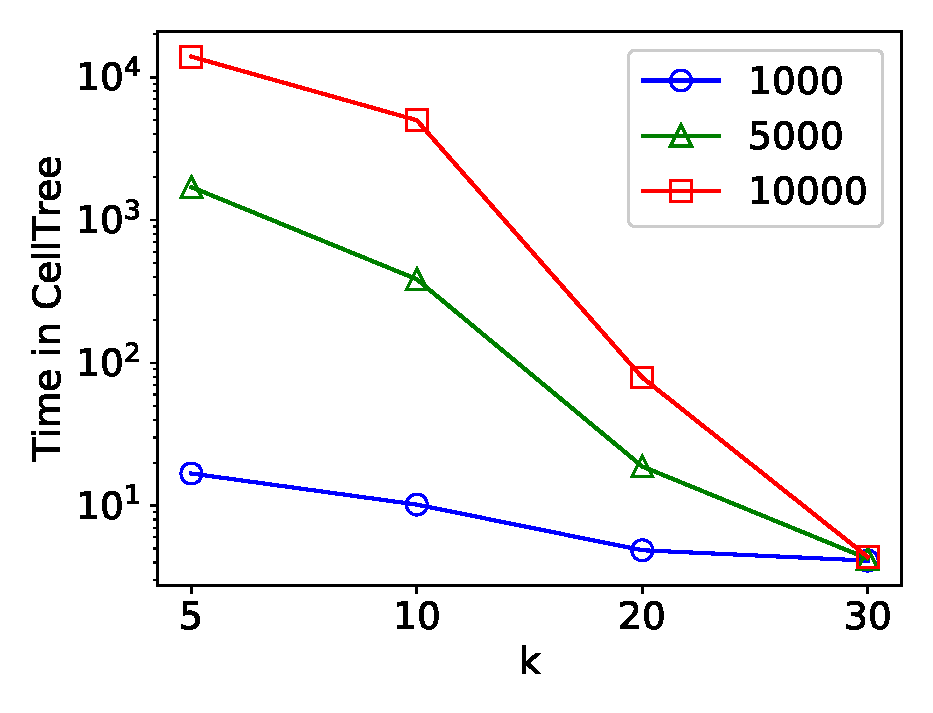
\includegraphics[width=.99\textwidth]{exp_topk1}
    \caption{Time spent in $CellTree$}
    \label{k_change_time}
  \end{subfigure}
  \caption{Effect of k (HOTEL)}
  \label{k_effect}
\end{figure}

Now we explore the impact of $k$. Our problem is to find a new product that rank as more as possible 
users' top $k$ as possible, and we have a prerequisite such that product dataset $P$ already 
covers a part of the users. With the increasing $k$, unchanged product dataset and 
user dataset, the products in dataset $P$ are to cover more users easily because the 
the threshold to be a user's top-$k$ is lowering down. With $P$ covering more users, no matter 
which of the lemmas
we propose or the baseline $CellTree$ approach will all greatly benefit from the reducing 
users. We show the experiment in Figure \ref{k_effect}. The y axis of Figure 
\ref{k_change_user_cnt} means the users number that we need to handle after removing 
the users that covered by $P$. We can see that user dataset with size 1000, 5000 or 10000, their 
uncovered users decrease exponentially with the change of k. And because of the decreasing
uncovered users, our response time also decreases exponentially.

\section{Effect of Product Dataset Distribution and B}

\begin{figure}[ht!]
  \centering
  \begin{subfigure}[b]{0.45\linewidth}
    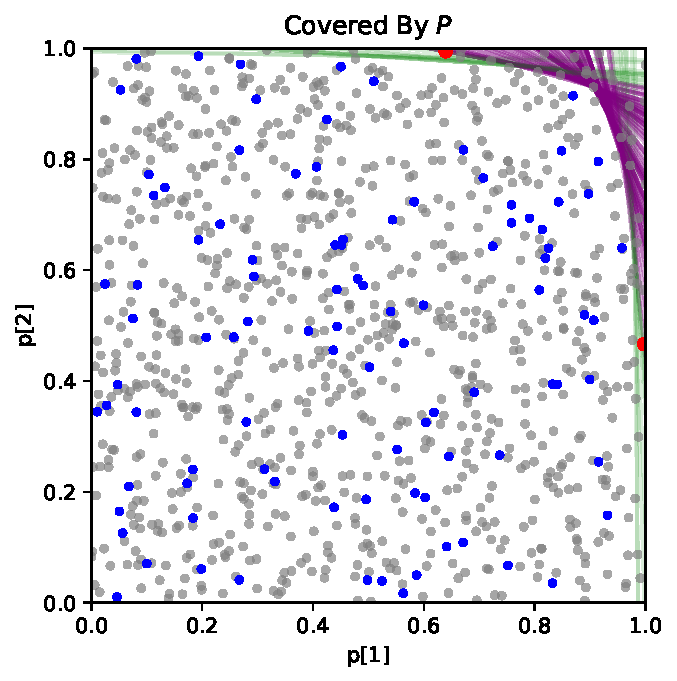
\includegraphics[width=.99\textwidth]{uni2dex0}
    \caption{Products and users covered by $P$}
    \label{cover_uni}
  \end{subfigure}
  %
  \begin{subfigure}[b]{0.45\linewidth}
    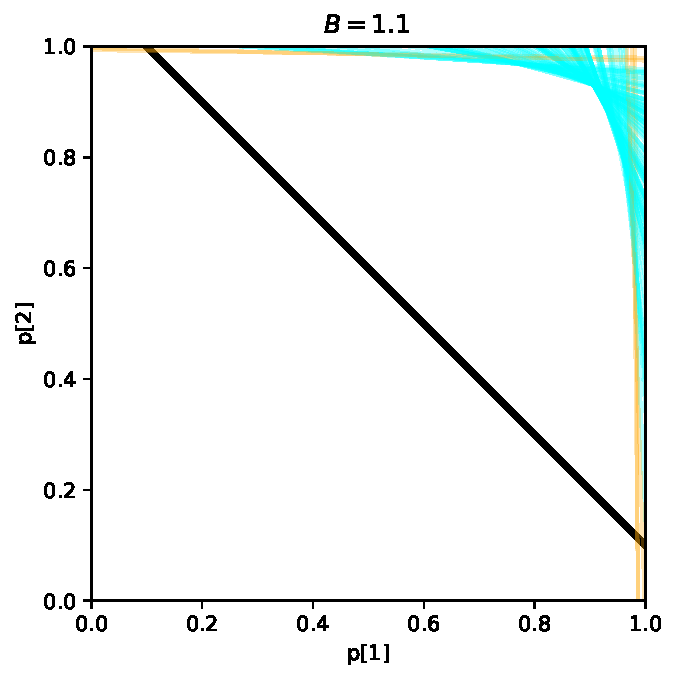
\includegraphics[width=.99\textwidth]{uni2dex1}
    \caption{Uniform, B=1.1}
    \label{it_uni_1_1}
  \end{subfigure}
  %
  \begin{subfigure}[b]{0.45\linewidth}
    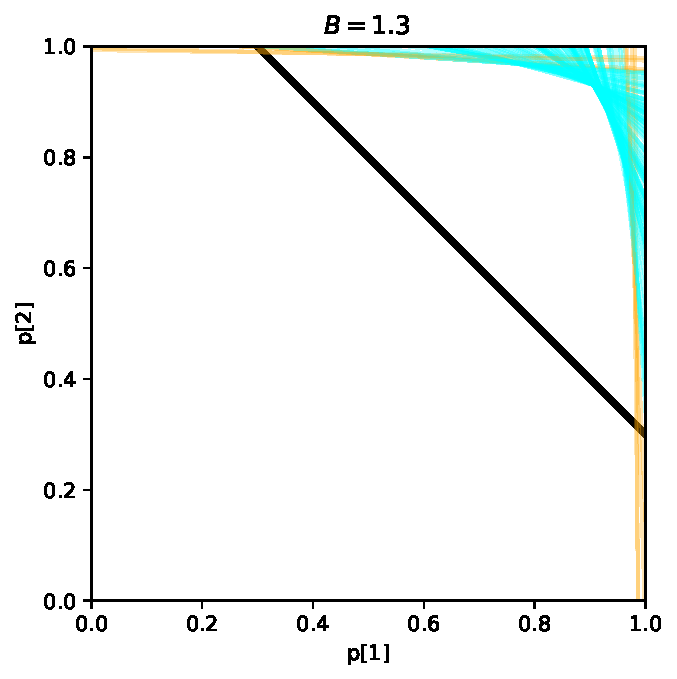
\includegraphics[width=.99\textwidth]{uni2dex2}
    \caption{Uniform, B=1.3}
    \label{it_uni_1_3}
  \end{subfigure}
  %      
  \begin{subfigure}[b]{0.45\linewidth}
    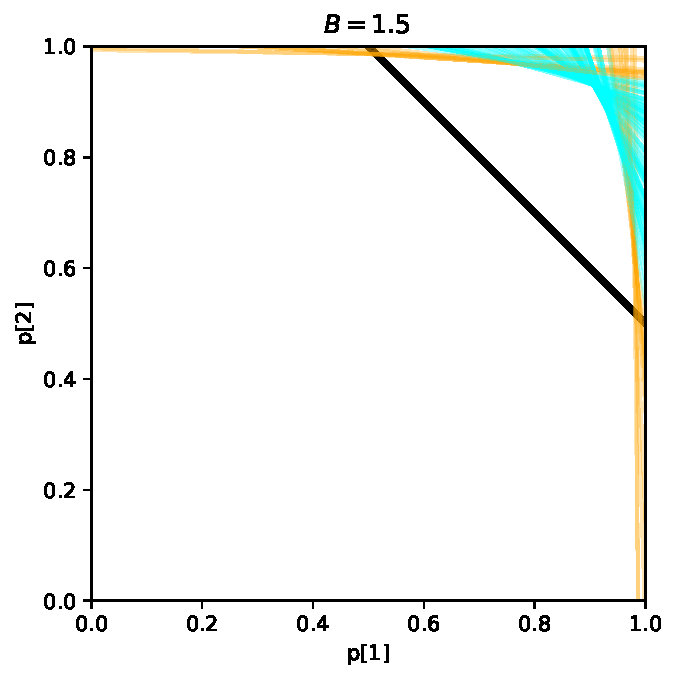
\includegraphics[width=.99\textwidth]{uni2dex3}
    \caption{Uniform, B=1.5}
    \label{it_uni_1_5}
  \end{subfigure}
  %
  \begin{subfigure}[b]{0.45\linewidth}
    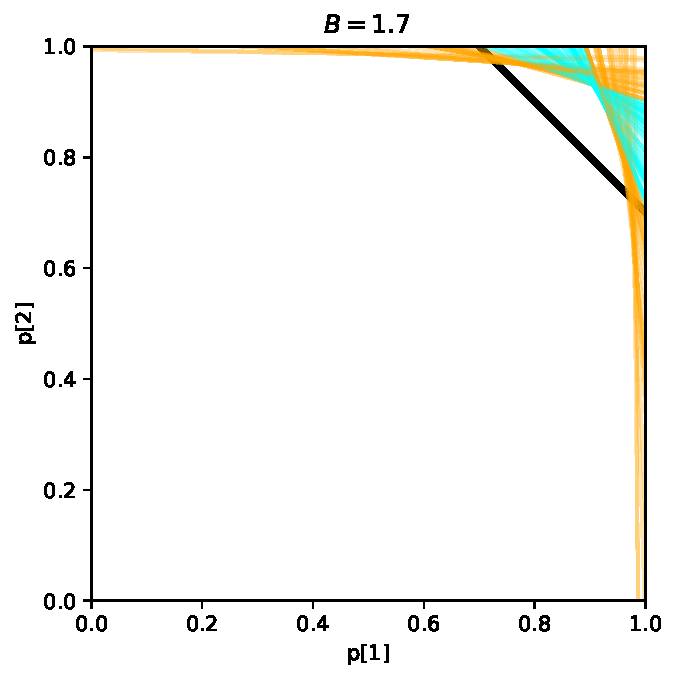
\includegraphics[width=.99\textwidth]{uni2dex4}
    \caption{Uniform, B=1.7}
    \label{it_uni_1_7}
  \end{subfigure}
  %      
  \begin{subfigure}[b]{0.45\linewidth}
    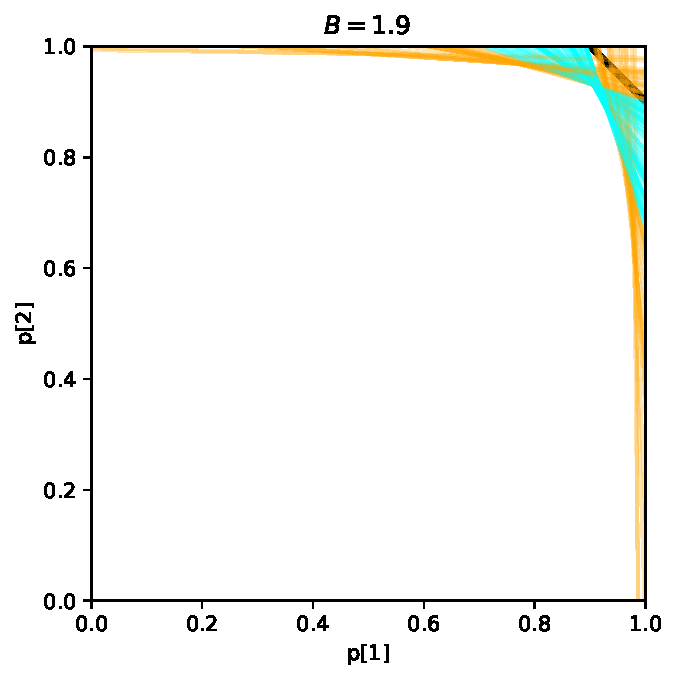
\includegraphics[width=.99\textwidth]{uni2dex5}
    \caption{Uniform, B=1.9}
    \label{it_uni_1_9}
  \end{subfigure}
  \caption{Effect of $B$ on uniform products}
  \label{uni_2d_demo}
\end{figure}



\begin{figure}[ht!]
  \centering
  \begin{subfigure}[b]{0.45\linewidth}
    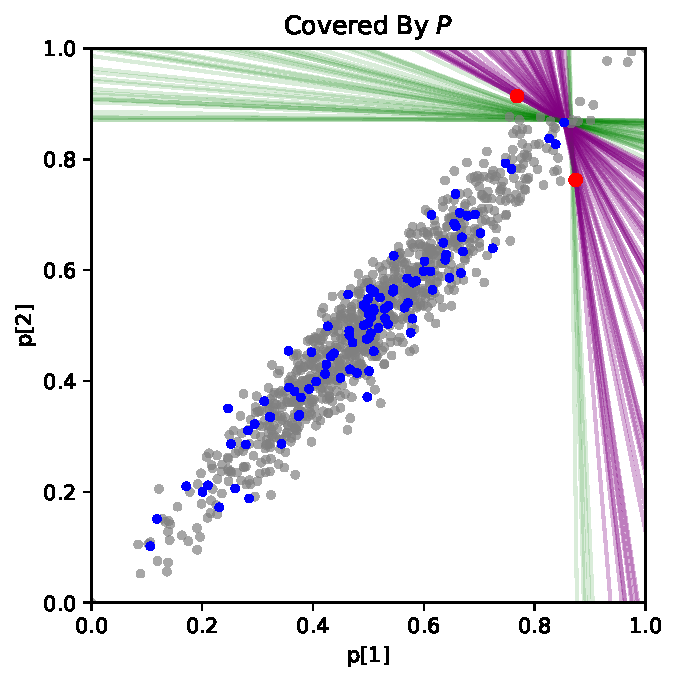
\includegraphics[width=.99\textwidth]{corr2dex0}
    \caption{Products and users covered by $P$}
    \label{cover_corr}
  \end{subfigure}
  %
  \begin{subfigure}[b]{0.45\linewidth}
    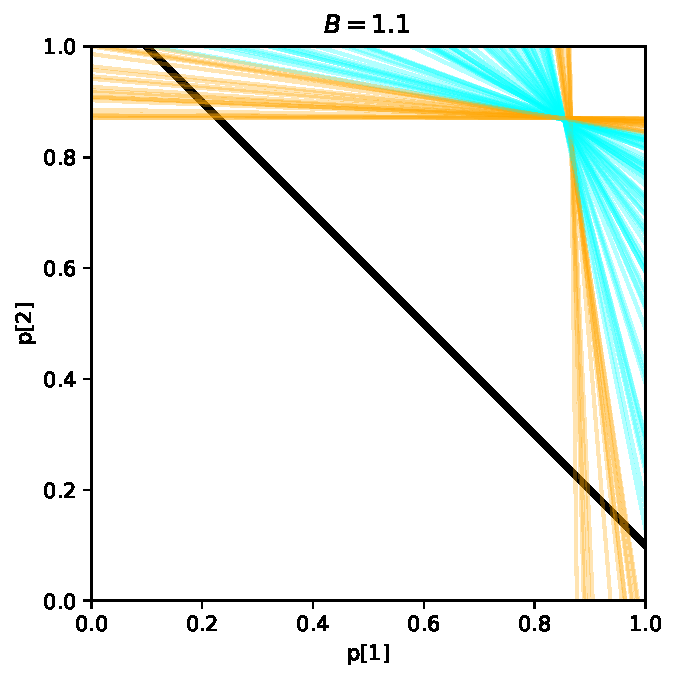
\includegraphics[width=.99\textwidth]{corr2dex1}
    \caption{Corr, B=1.1}
    \label{it_corr_1_1}
  \end{subfigure}
  %
  \begin{subfigure}[b]{0.45\linewidth}
    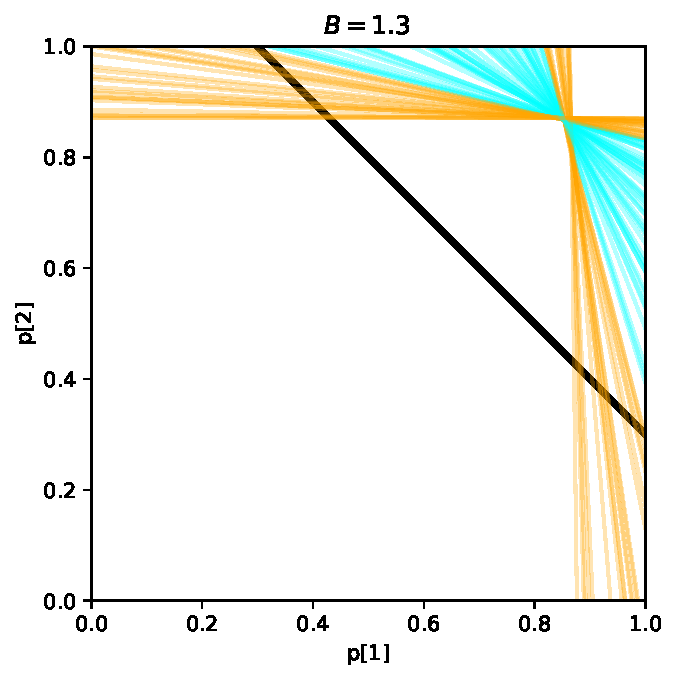
\includegraphics[width=.99\textwidth]{corr2dex2}
    \caption{Corr, B=1.3}
    \label{it_corr_1_3}
  \end{subfigure}
  %      
  \begin{subfigure}[b]{0.45\linewidth}
    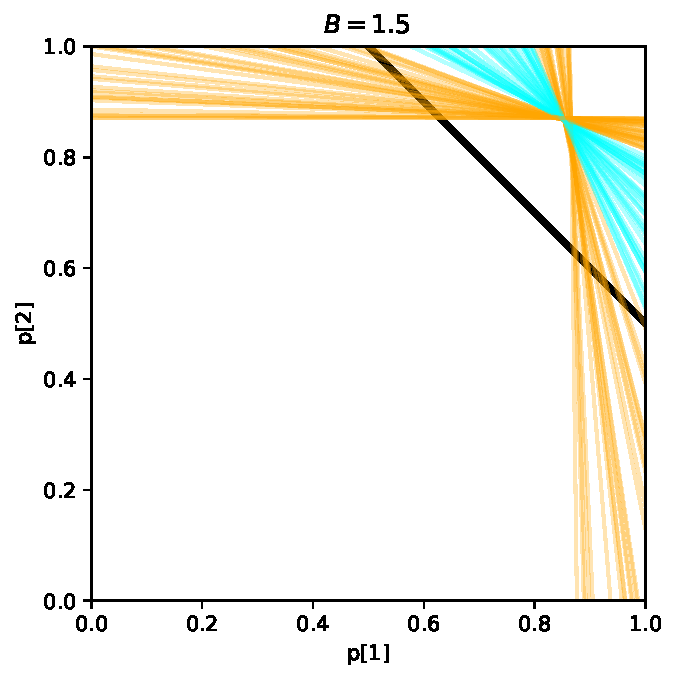
\includegraphics[width=.99\textwidth]{corr2dex3}
    \caption{Corr, B=1.5}
    \label{it_corr_1_5}
  \end{subfigure}
  %
  \begin{subfigure}[b]{0.45\linewidth}
    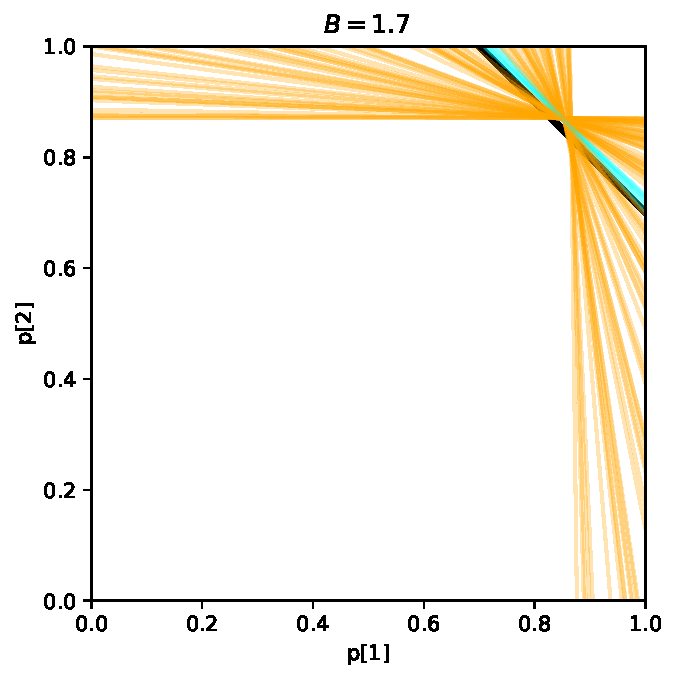
\includegraphics[width=.99\textwidth]{corr2dex4}
    \caption{Corr, B=1.7}
    \label{it_corr_1_7}
  \end{subfigure}
  %      
  \begin{subfigure}[b]{0.45\linewidth}
    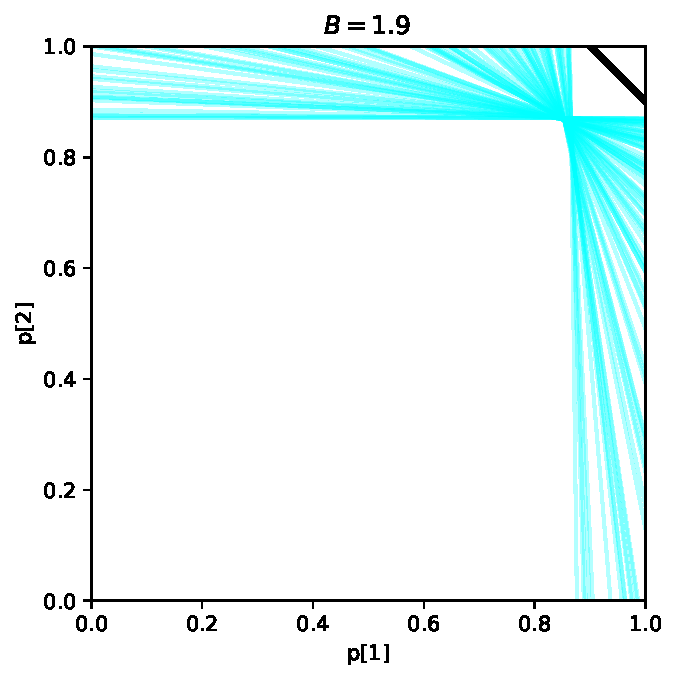
\includegraphics[width=.99\textwidth]{corr2dex5}
    \caption{Corr, B=1.9}
    \label{it_corr_1_9}
  \end{subfigure}
  \caption{Effect of $B$ on corr products}
  \label{corr_2d_demo}
\end{figure}

\begin{figure}[ht!]
  \centering
  \begin{subfigure}[b]{0.45\linewidth}
    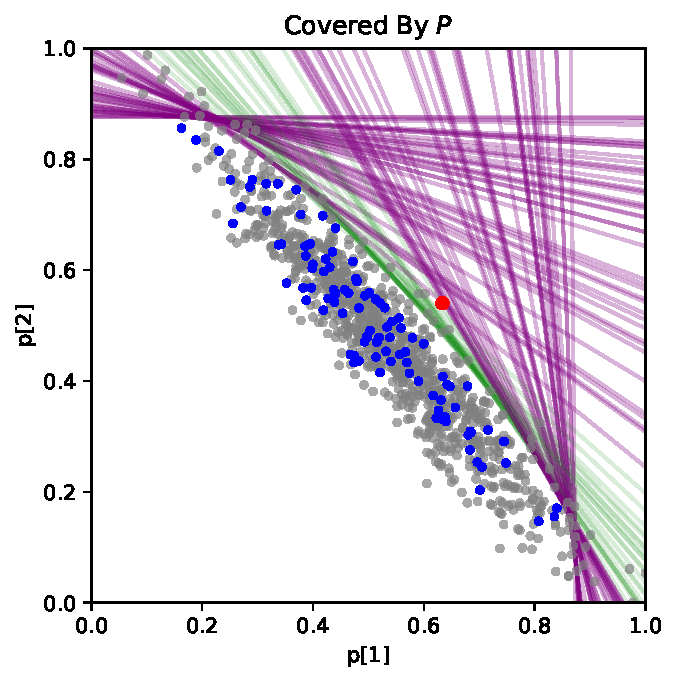
\includegraphics[width=.99\textwidth]{anti2dex0}
    \caption{Products and users covered by $P$}
    \label{cover_anti}
  \end{subfigure}
  %
  \begin{subfigure}[b]{0.45\linewidth}
    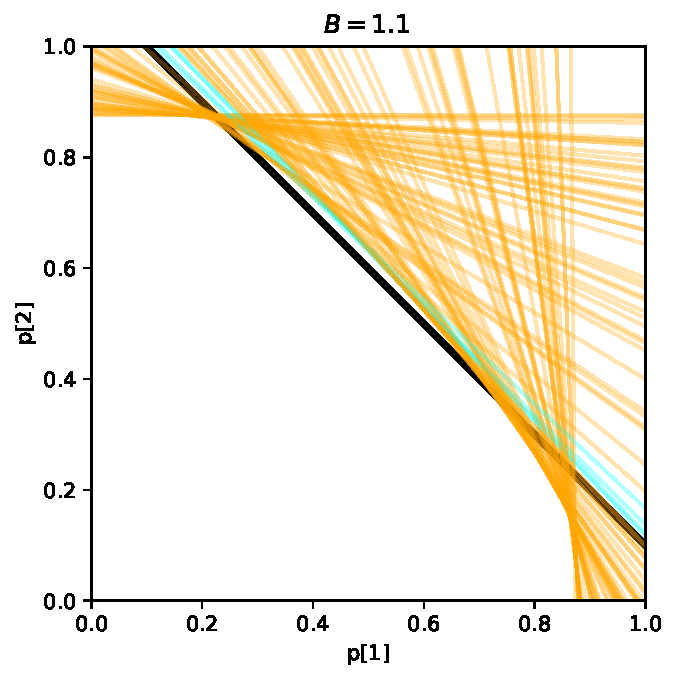
\includegraphics[width=.99\textwidth]{anti2dex1}
    \caption{Anti, B=1.1}
    \label{it_anti_1_1}
  \end{subfigure}
  %
  \begin{subfigure}[b]{0.45\linewidth}
    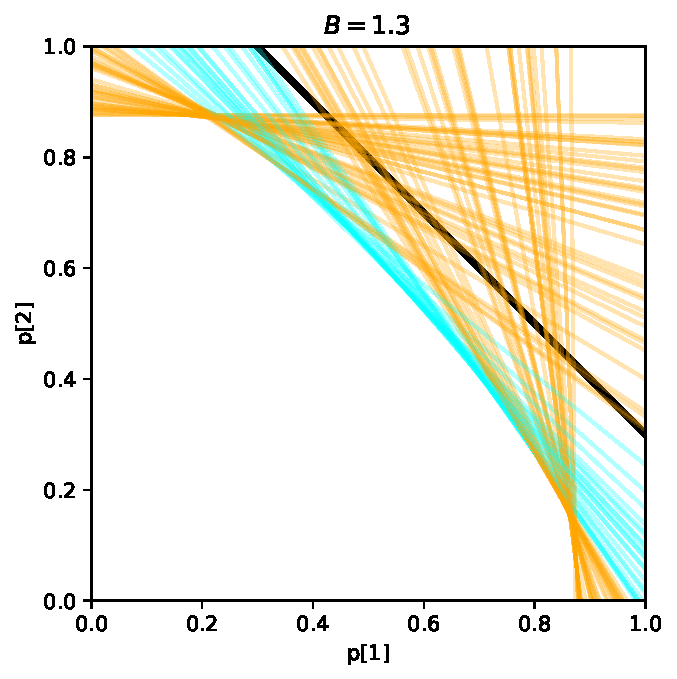
\includegraphics[width=.99\textwidth]{anti2dex2}
    \caption{Anti, B=1.3}
    \label{it_anti_1_3}
  \end{subfigure}
  %      
  \begin{subfigure}[b]{0.45\linewidth}
    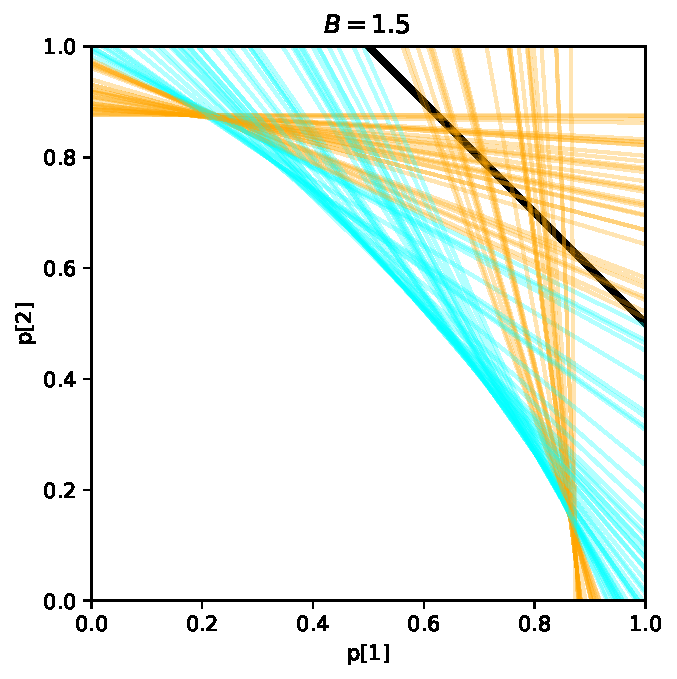
\includegraphics[width=.99\textwidth]{anti2dex3}
    \caption{Anti, B=1.5}
    \label{it_anti_1_5}
  \end{subfigure}
  %
  \begin{subfigure}[b]{0.45\linewidth}
    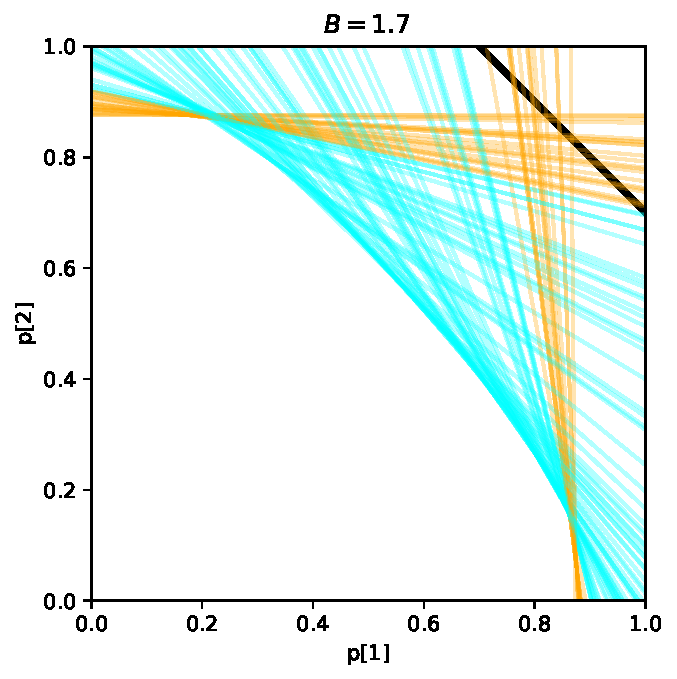
\includegraphics[width=.99\textwidth]{anti2dex4}
    \caption{Anti, B=1.7}
    \label{it_anti_1_7}
  \end{subfigure}
  %      
  \begin{subfigure}[b]{0.45\linewidth}
    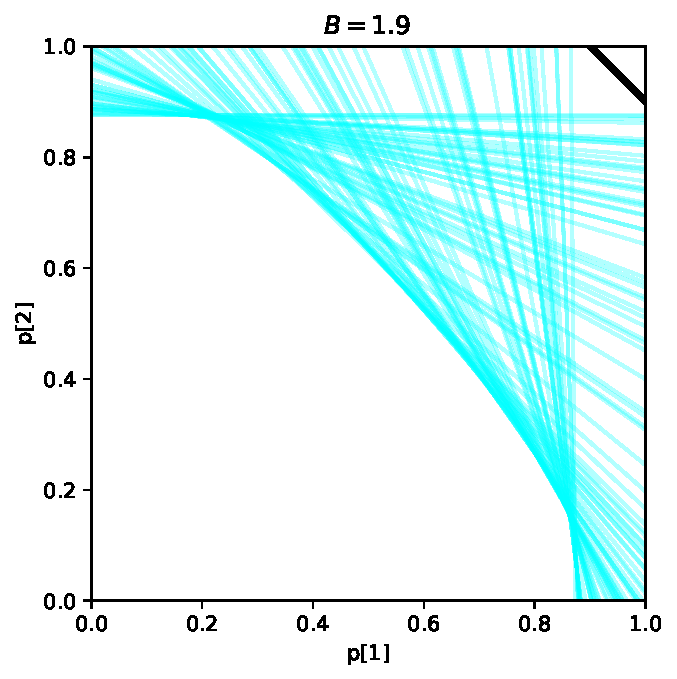
\includegraphics[width=.99\textwidth]{anti2dex5}
    \caption{Anti, B=1.9}
    \label{it_anti_1_9}
  \end{subfigure}
  \caption{Effect of $B$ on anti products}
  \label{anti_2d_demo}
\end{figure}

To straight forward presents our algorithm and shows the interesting finding in
experiments, we use a 2d experiment and visualize it as in Figure 
\ref{uni_2d_demo}, \ref{corr_2d_demo} and \ref{anti_2d_demo}.

First of all, the users are all generated uniformly from $w[1]+w[2]=1$.

To explain Figure \ref{uni_2d_demo}, \ref{corr_2d_demo} and \ref{anti_2d_demo}, we
take \ref{cover_uni} as an example, this figure is drawn in product space. 
Product dataset $D$ consists with the grey, blue and red points
; product dataset $P$ consists with the blue and red points; the red points are the points that 
each of them at least covers one user.  Specially, 
we have to expand the size of red points to clearly show them. We can see the red points
of Figure \ref{cover_uni} at about $(0.9, 0.9)$ and $(0.95, 0.8)$.
The lines are all $w_i\dot p=S_{ik}$. The blue lines mean the corresponding $w_i\dot p=S_{ik}$ of users 
that covered by $P$ and the rest users' halfspaces are orange lines. From Figure 
\ref{it_uni_1_1} to Figure \ref{it_uni_1_9}, the bold black line means 
the constraint $\Sigma_{i=1}^d p[i]\leq B$ when $B$ equals 1.1, 1.3, 1.5, 1.7, 1.9 respectively.
The orange lines mean the $w_i\dot p=S_{ik}$ that intersects with constraint and the blues aren't
intersect with constraint. 

In Figure \ref{cover_uni}, because the distribution of products is uniform so 
for each user weight vector $w_i$, there is a proper product $p_{wi}$ nearby the extend of
$w_i$ ranks top-$k$ for it. And because the halfspace $w_i\cdot p=S_{ik}$ getting through the point $p_{wi}$,
so the lower bounds of $w_i\dot p=S_{ik}$ makes a smooth curve along $p[2]=1$ and
$p[1]=1$. From Figure \ref{it_uni_1_1} to Figure \ref{it_uni_1_9}, the number of the halfspaces
that intersect with constraint increases with the increasing $B$ because more and more 
products become some of the users' top-$k$ and so as will more halfspaces be there.


In Figure \ref{cover_corr}, the red point is around $(0.9, 0.9)$. In correlated 
distribution products as shown in \ref{cover_corr}, almost all the products that 
rank $k$ for users are at the location that is closed to $(1, 1)$. Because the 
halfspaces will get through the points that rank exactly $k$ and
products ranking $k$ are almost the same or very closed to each other, it seems all
halfspaces intersect at one point. Be careful that they aren't intersect at exact
one point and it looks so just because of the size of figure we can show. The halfspaces
that intersect with constraint will gradually increase and at a special B decrease
suddenly as we can see from Figure \ref{it_corr_1_1} to Figure \ref{it_corr_1_9}.

In Figure \ref{cover_anti}, the red points are about at $(0.1, 0.95)$, $(0.3, 0.8)$, $(0.8, 0.3)$.
The products that exactly rank $k$ for users concentrate on $(0.2, 0.9)$ and $(0.9, 0.2)$.
This could be explained by the Lemma 4 of $k-hit query$, which says that for any 
weight vector $w$ if only a point $p_ix$ inside the convex hull made by 
$P_i=\{p_i1, p_i2, ..., p_{i(x-1)}\}$, then there must be a point in $P_i$
such that its dot product with $w$ is higher than $p_ix$'s. 
For our case of anti-correlated distribution products, most of products are between
the points nearby $(0, 1)$ and $(1, 0)$ which means for any weight vector, its top-$k$
is nearby $(0, 1)$ or $(1,0)$ when $k$ is small and $card(D)$ is also large. Therefore,
in Figure \ref{anti_2d_demo} we can see most of halfspaces getting through $(0.2, 0.9)$ and $(0.9, 0.2)$
which is closed to $(0,1)$ or $(1, 0)$. With the increasing of $B$, the number of 
halfspaces that 
intersect with constraint suddenly increases and then gradually decreases. 


In Figure \ref{uni_2d_demo}, \ref{corr_2d_demo} and \ref{anti_2d_demo}, we show the process of our
algorithm to solve $kCRM$. Firstly, remove the users that covered by $P$. Remove the 
halfspaces $w_i\cdot p=S_{ik}$ that doesn't intersect with constraint. Change
the insertion order of halfspaces by some heuristic. Use $CellTree$
proposed in $kSPR$ to find the region that cover the most of the rest of users.
During the process in $CellTree$, prune the tree nodes with lower bound of optimal
solution.



\begin{figure}[hbt!]
  \centering
  \begin{subfigure}[b]{0.8\linewidth}
    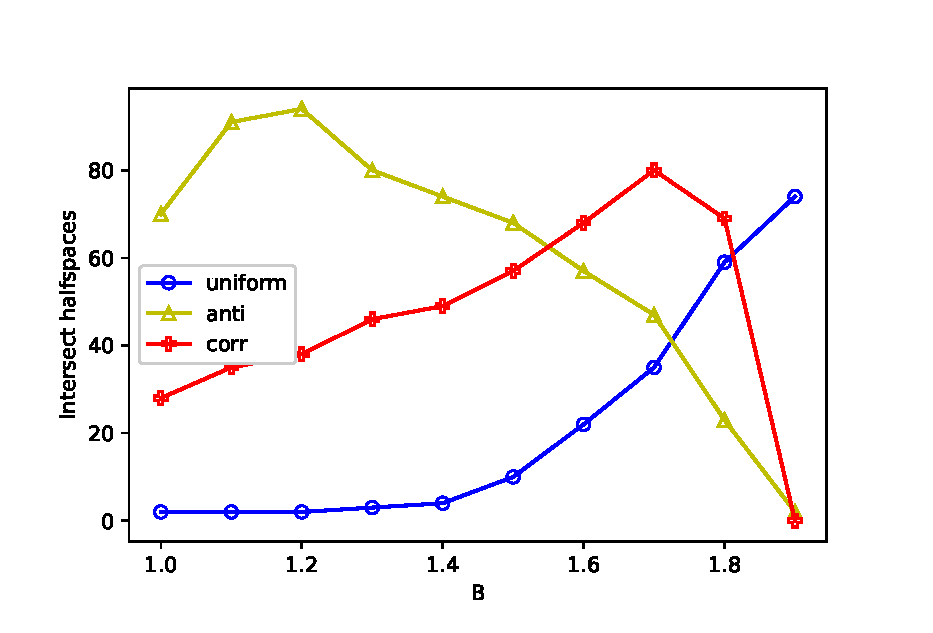
\includegraphics[width=.99\textwidth]{inters_B}
  \end{subfigure}
  \caption{No. of halfspaces intersect with constraint}
  \label{inters_B}
\end{figure}

Figure \ref{inters_B} shows the exact changes of halfspaces. 

For uniform generated
products, intersect halfspaces increases gradually. If the new proposed product wants 
to cover as more user as possible, its attributes should balance and all with high
values. And if the new product is already a top-$k$ option for some users, it is 
hard for it to cover more because each aspect of it is already high and the cost of
develop such product is too high to afford or too hard to realize. But still, we
could introduce the product that only satisfies some kind of users. For example,
to cover users that care more about $p[1]$, we can introduce the new product as
$p=(1, 0.5)$ under the constraint $p[1]+p[2]\leq 1.5$. 

For correlated generated products,
intersect halfspace increases gradually and then suddenly decrease. For this kind of
product distribution, it is also recommended to introduce new products that with 
high value in some attribute. It is easy for correlated products to introduce a new product
that cover all of the users since there are already existing several products 
cover all of users but for uniformly products it is not likely to find product that 
cover all users.


For anti-correlated
generated products, intersect halfspaces firstly increases for a short time and then
gradually decreases. In real world, most of the product datasets are based on this 
distribution, such as $HOTEL$ and $HOUSE$ data proposed in this paper.  For each
attribute, there is a certain value that if the product's corresponding attribute
exceeds it then this product will cover a kind of users. To cover different kinds 
of users, the new product has to balance each attribute. Because in real world
the users that favor in each attribute are unbalance. For example, there are more 
users prefer
computers with powerful computation ability than with large memory. Consider the case
$P=\emptyset$, to cover more users the new product just needs to with high value
in the attribute that considered more important by most users. When $P\neq \emptyset$, 
as we can see from Figure \ref{cover_anti}, to covered all of the rest user(the orange lines), we need
to introduce products such as $\{(0.1, 0.95), (0.95, 0.1)\}$. To covered them by a single
product, we need a product for example no worse than $(0.9, 0.7)$. But in realistic, 
the option decision maker isn't likely to introduce such single product under the 
limitation of technology, money and other factors. The best strategy is to firstly 
introduce product $(0.95,0.1)$ and then is $(0.1, 0.95)$. It is hard to cover
all the users and company should take good evaluation of market so as to step by
step make more profits.


 
  
\chapter*{CONCLUSION}
\label{chap:conclusion}
Motivated by the need of introducing new product, we proposal our problem kCRM, 
which is aim to find the exact optimal solution that covers the most rest users which
product dataset $P$ can't cover. We use data structure $CellTree$ introduced in 
$kSPR$ as our baseline. Then we base on the relationship between constraint and user 
insertion
halfspace to prune unrelated users and get lower bound of optimal solution to prune
the nodes in $CellTree$. Besides, we change the insertion order of user halfspaces 
to more efficiently process insertion reducing the possible useless nodes.
In our paper, we use experiments to show our optimization for the baseline did improve it
a great deal and we find some inner connection between efficiency of our approach 
and constraint. For the future work, we can perform further study the effect of insertion
order of halfspaces to more efficiently solve $kCRM$ and so that we can deal with larger
user datasets.      


%%%%%%%%%%%%%%%%%%%%%%%%%%%%%%
%% 附件部分
%%%%%%%%%%%%%%%%%%%%%%%%%%%%%%
\backmatter
  %结语
  
  % 参考文献
  % 使用 BibTeX
  % 选择参考文献的排版格式。注意ustcbib这个格式不保证完全符合要求,请自行决定是否使用
  \bibliographystyle{sustcbib}%{GBT7714-2005NLang-UTF8}
  %\bibliographystyle{IEEEtran}
  \bibliography{bib/tex}
  \nocite{*} % for every item
  % 不使用 BibTeX
  %\include{chapter/bib}
  % 附录,没有请注释掉
  %\begin{appendix}

  %\chapter{Experiment Results}
\label{chap:appA}
Some descriptions here.
\section{Subsection}

  
  %\end{appendix}
  \begin{thanks}
四年的光阴不长不短, 
在春节辅导员顺路接送回家,
跟校学生会文娱部的大家组织过很多活动有过许多快乐的时光,
在风景美丽的校园上体育课,
生物课老师对我差劲英语的包容, 
物理课老师对我不耐烦的教导,
细心认真的Stéphane Faroult带领我走入计算机专业,
时常上课给同学人生建议的王琦老师,
书院导师杨柳青给与我们生活上的指导, 
书院班主任史玉回老师给我们分享的自己的人生经历,
Hisao教授带领我进入科研, 
唐博教授教懂我如何做项目, 
邵宣杰同学四年中对我数学上的帮助,
经常一起谈笑风生的黄旭以及张思宇同学, 
华为实习期间一直帮助我的工作导师苏林达, 组长林吉生以及同事王玮,
有幸遇到各位优秀DBGroup@SUSTech的成员,
感谢学校给与的丰厚资助,
强大的师资与硬件,
非常感谢让我一路上经历的这一切美好与困难。
最感谢的是我的父母, 在我大学期间我体会到学校无微不至的关怀, 真诚的关心, 认真的付出 , 
这些我都将铭记在心。
\vskip 18pt

\begin{flushright}

李可明

2020年5月20日

\end{flushright}

\end{thanks}

\end{document}
